\documentclass[11pt,a4paper]{article}

\usepackage[utf8]{inputenc}
\usepackage[T1]{fontenc}
\usepackage{amsmath,amssymb,amsthm}
\usepackage{mathtools}
\usepackage{bm}
\usepackage[margin=2.5cm]{geometry}
\usepackage{natbib}
\usepackage{hyperref}
\usepackage{booktabs}
\usepackage{enumitem}
\usepackage{appendix}
\usepackage{graphicx}
\graphicspath{{figures/}}
\usepackage{float}

\numberwithin{equation}{section}

\pagestyle{myheadings}
\markright{MV Allocation under RS Jump-Diffusions}

%for submission
\usepackage{setspace}\doublespacing

% Theorem environments
\newtheorem{theorem}{Theorem}[section]
\newtheorem{proposition}[theorem]{Proposition}
\newtheorem{lemma}[theorem]{Lemma}
\newtheorem{corollary}[theorem]{Corollary}
\newtheorem{definition}[theorem]{Definition}
\newtheorem{remark}[theorem]{Remark}
\newtheorem{assumption}[theorem]{Assumption}
\newtheorem{problem}[theorem]{Problem}

% Commands
\newcommand{\E}{\mathbb{E}}
\newcommand{\Var}{\mathrm{Var}}
\newcommand{\Prob}{\mathbb{P}}
\newcommand{\R}{\mathbb{R}}
\newcommand{\N}{\mathbb{N}}
\newcommand{\F}{\mathcal{F}}
\newcommand{\G}{\mathcal{G}}
\newcommand{\Lp}{\mathcal{L}}
\newcommand{\Ov}{\mathcal{O}} % Overshoot mass (avoids big-O collision)
\newcommand{\dd}{\mathrm{d}}
\newcommand{\SR}{\mathrm{SR}}
\newcommand{\ie}{\textrm{i.e.,}}
\newcommand{\eg}{\textrm{e.g.,}}
\newcommand{\cf}{\textrm{cf.}}
\newcommand{\ind}{\mathbf{1}}
\DeclareMathOperator{\diag}{diag}
\DeclareMathOperator{\sgn}{sgn}
\DeclareMathOperator{\re}{Re}

\title{\textbf{Dynamic Mean--Variance Portfolio Allocation \\ under Regime-Switching Jump-Diffusions \\ with Absorbing Barriers and Distribution Matching}}

\author{Artur Sepp\thanks{LGT Private Banking, Zurich. Email: artur.sepp@lgt.com}}

\date{7 April 2026}

\begin{document}

\maketitle

\begin{abstract}
We study the continuous-time dynamic mean--variance (MV) portfolio 
allocation problem when the risky asset follows a two-state 
regime-switching process with exponentially distributed jumps occurring 
at regime transitions. The value function admits a regime-conditional 
quadratic representation, yielding a coupled system of nonlinear Riccati 
ordinary differential equations whose optimal feedback policy retains the 
Merton--Lipton structure---the Merton ratio adjusted by a goal-seeking 
funding ratio---in each regime.
We introduce an absorbing wealth floor for capital preservation and 
develop a Laplace transform framework employing Arrow--Debreu state prices 
in the Laplace domain. The stopped wealth distribution has two components 
absent in the pure diffusion case: regime-dependent stopping probabilities 
and jump overshoot below the floor.
We formulate the inverse problem of matching a target terminal wealth 
distribution using mixtures of stopped strategies across asset classes and 
show that the family of achievable distributions approximates target distributions in the Wasserstein-1 topology. Numerical examples 
illustrate the framework for a three-asset-class portfolio (bonds, equity, 
private equity) calibrated to typical capital market assumptions.
\end{abstract}

\medskip
\noindent\textbf{Keywords:} Dynamic mean--variance allocation; regime-switching jump-diffusion; exponential jumps; coupled Riccati equations; first-passage time; Laplace transform; barrier options; terminal wealth distribution; distribution matching.

\medskip
\noindent\textbf{MSC 2020:} 91G10, 93E20, 60J28, 60G40, 49L20.

\medskip
\noindent\textbf{JEL:} G11, C61, C58.


%% ============================================================================
%% SECTION 1: INTRODUCTION
%% ============================================================================
\section{Introduction}\label{sec:intro}

\citet{ZhouLi2000} formulated an important problem of continuous-time mean--variance (MV) portfolio selection as a stochastic linear-quadratic control problem. For an asset following geometric Brownian motion (GBM), \citet{Lipton2001} derived an elegant closed-form solution: the optimal allocation is the Merton ratio $(\mu - r)/\sigma^2$ multiplied by a goal-seeking factor $(1/F_t - 1)$ depending on the funding ratio $F_t = \Pi_t / \Pi^*(t)$, where $\Pi_t$ and $\Pi^*(t)$ are the current and target value of the wealth process. \citet{ZhouYin2003} \citep[see also][]{ChenYaoYin2008,Xie2008} extended the diffusion model to regime-switching markets, where all parameters are modulated by a finite-state Markov chain, and derived explicit efficient frontiers via two systems of linear ordinary differential equations (ODEs) using the stochastic Linear-Quadratic (LQ) framework. \citet{SotomayorCadenillas2009} derived explicit consumption--investment solutions under regime switching with CRRA utility. The MV problem with regime-switching-induced jumps was recently treated by \citet{ShiXu2025}, who derive coupled nonlinear Riccati equations and prove their solvability. 


Portfolio optimisation with drawdown constraints was initiated by \citet{GrossmanZhou1993}, who showed that optimal investment is proportional to the surplus above a stochastic floor. \citet{ContTankov2009} analysed the gap risk of constant proportion portfolio insurance (CPPI) strategies---where the allocation is a constant multiple of the cushion $\Pi - L$---under jump-diffusions, deriving analytical formulas for the floor-breach probability and loss distribution. Our three-component decomposition of the stopped wealth distribution (survival, floor atom, jump overshoot) is related to the diffusion--jump risk decomposition of intra-horizon expected shortfall developed by \citet{FarkasVasiljevic2021}.  

 

Naturally, based on the empirical evidence, jump-diffusions provide more robust framework for analysis of the wealth dynamics. \citet{DangForsyth2014} solve the pre-commitment mean-variance problem under \cite{Kou2002} double-exponential jump-diffusion numerically and show that jumps significantly affect the efficient frontier. However, stopping problems under jump-diffusions are challenging to solve for analytical frameworks. The Laplace transform approach to barrier options applied to credit risk under exponential jumps was developed by \citet{Lipton2001assets}, extended by \citet{Sepp2004} to (non-switching) double-exponential jump-diffusions and by \citet{Sepp2006} to stochastic volatility. We extend this framework to the regime-switching setting. Alternative transform methods for barrier options under L\'evy processes include the Wiener--Hopf approach of \citet{BoyarchenkoLevendorskii2012} and the Hilbert transform method of \citet{FengLinetsky2008}. The first-passage problem under regime-switching with jumps has been studied via Wiener--Hopf factorisation \citep{JiangPistorius2008} and martingale methods \citep{SiuEtAl2014}. Our PIDE-based approach provides explicit formulas for all quantities needed in the portfolio context. 


In this paper we address several features of real markets and wealth planning extending the existing formulations.


First, we assume jumps at regime transitions. Empirical evidence shows that equity prices experience sharp declines when markets shift from bullish to bearish regimes, and vice versa \citep{Hamilton1989}. Standard regime-switching models (\citealt{ZhouYin2003} and followers) treat the Markov chain as independent of the price process, missing this phenomenon.  \citet{ShiXu2025} addressed this by adding independent Poisson jumps whose intensities are modulated by the regime. We take a more parsimonious approach: in our model, jumps occur precisely at regime transitions---the crash is the regime switch, not a separate event. This yields a lower-dimensional system (a sixth-order characteristic polynomial versus higher order for independent jumps) while capturing the empirically observed simultaneity of market dislocations and regime changes. The trade-off is that intra-regime jumps are excluded; extending to 
independent jump arrivals with regime-dependent intensities increases 
the characteristic polynomial order beyond six.


Second, we incorporate wealth floors and stopped distributions. In practice, portfolios may be frequently managed with explicit drawdown limits or wealth floors \citep{GrossmanZhou1993}. The MV problem with a non-negativity (bankruptcy prohibition) constraint was solved by \citet{BieleckiJinPliskaZhou2005}, but the terminal wealth distribution under a general floor constraint is fundamentally different from the unconstrained case: it includes an atom at the floor level and, with jumps, a continuous component below the floor from overshoot. The dynamic MV problem with a wealth floor has not, to our knowledge, been treated in a regime-switching jump-diffusion framework.

Third, we explicitly design the target of wealth distribution. The goal-based investing paradigm requires not merely an efficient frontier but a specific shape of the terminal wealth distribution matching the investor's preferences.


This paper addresses all three features in a unified framework. Our contributions are the following.

Firstly, we establish that the MV value function under a two-state regime-switching model with exponential transition jumps admits a regime-conditional quadratic form (Theorem~\ref{thm:quadratic_ansatz}). The resulting coupled nonlinear Riccati system has a unique global solution (Theorem~\ref{thm:riccati_existence}), and the associated feedback policy is optimal (Theorem~\ref{thm:verification}). The optimal allocation in each regime retains the Merton--Lipton structure with regime-dependent effective Sharpe ratios (Corollary~\ref{cor:optimal_policy}).

Secondly, we develop a Laplace transform framework for first-passage problems under the regime-switching jump-diffusion (Section~\ref{sec:laplace}). Arrow--Debreu state prices in the Laplace domain satisfy a coupled system of ordinary integro-differential equations (OIDEs) whose solutions are determined by a sixth-order characteristic polynomial (Theorem~\ref{thm:char_poly}) with three positive and three negative roots (Lemma~\ref{lem:root_structure}). The unbounded and bounded (barrier) problems admit explicit solutions in the Laplace domain (Theorem~\ref{thm:unbounded_solution} and Theorem~\ref{thm:bounded_solution}), from which survival probabilities (Corollary~\ref{cor:survival}), first-passage densities (Corollary~\ref{cor:hitting}), and conditional moments (Theorem~\ref{thm:cond_moments}) are obtained via numerical Laplace inversion. We characterise the stopped terminal wealth distribution as a mixture of three components: survival paths, diffusion-hitting paths (floor atom), and jump-overshoot paths (Proposition~\ref{prop:three_components}). All components are computable from the Laplace framework.

Thirdly, our framework in Section~\ref{sec:stopped} generalises the CPPI analysis of \citet{ContTankov2009} in two directions: the allocation is MV-optimal rather than proportional to the cushion (the Merton--Lipton policy \eqref{eq:optimal_w} is concave in $\Pi$, not linear), and the dynamics include regime switching.  The three-component decomposition of the stopped wealth (Proposition~\ref{prop:three_components}) extends the Cont--Tankov gap-risk decomposition to the regime-switching setting: their floor-breach probability corresponds to our total stopping probability $p_L$, and their loss distribution (from jump overshoot) corresponds to our Component~(c).  The key difference is that the MV-optimal allocation adapts dynamically to the funding ratio, while CPPI uses a fixed multiplier.  

Lastly, we formulate the inverse problem of fitting a target terminal wealth distribution, as specified by an investor, by mixtures of stopped strategies across asset classes (Section~\ref{sec:inverse}). Under mild conditions, we show that the family of achievable distributions is dense in the Wasserstein-1 topology (Proposition~\ref{prop:achievable}).  We develop a structured parameterisation of this problem (Section~\ref{sec:opportunity}): the advisor's constraints reduce the weight simplex to a one-parameter curve (bond weight), and the monotonicity of the implied return (Proposition~\ref{prop:r_impl_monotone}) reduces the investor's decision to a scalar selection.  The resulting expected allocation to the risky portfolio decreases endogenously over the investment horizon---an analytically derived de-risking glide path whose rate depends on the consumption gap $\max(0, c - r)$.

The paper is organised as follows. Section~\ref{sec:model} introduces the regime-switching model. Section~\ref{sec:mv} formulates and solves the MV problem. Section~\ref{sec:stopped} defines the stopped wealth process, establishes the flat-barrier reduction, and identifies the three components of the terminal wealth distribution. Section~\ref{sec:laplace} develops the Laplace transform framework. Section~\ref{sec:terminal_dist} derives the terminal wealth density and analytical conditional moments. Section~\ref{sec:numerics} provides quantitative illustrations. Section~\ref{sec:opportunity} develops the investment opportunity set framework and analyses the resulting allocation dynamics. Proofs are collected in the Appendices. The companion Python package \texttt{GoalBasedAllocation} 
\citep{SeppGBA2026} implements the full analytical framework---Riccati 
ODE system, Laplace-domain density and survival computations, 
and Monte Carlo validation---and reproduces all figures and tables 
in this paper.



%% ============================================================================
%% SECTION 2: MODEL
%% ============================================================================
\section{Model and Preliminaries}\label{sec:model}


Let $(\Omega, \F, \{\F_t\}_{t \geq 0}, \Prob)$ be a filtered probability space supporting a standard Brownian motion $W = \{W_t\}_{t \geq 0}$ and a continuous-time Markov chain $\chi = \{\chi_t\}_{t \geq 0}$ with state space $\{1,2\}$ and generator matrix
\begin{equation}\label{eq:generator}
\Lambda = \begin{pmatrix} -\lambda^{[12]} & \lambda^{[12]} \\ \lambda^{[21]} & -\lambda^{[21]} \end{pmatrix},
\end{equation}
where transition intensities $\lambda^{[12]}, \lambda^{[21]} > 0$. We assume $W$ and $\chi$ are independent. Regime~1 (growth) and regime~2 (stress) are interpreted as the normal and stressed market regimes, respectively. We refer to the transition $1 \to 2$ as a crash and $2 \to 1$ as a recovery.



\subsection{Asset dynamics}\label{sec:asset}

The risky asset price $S_t$ follows the regime-switching dynamics:
\begin{equation}\label{eq:asset_sde}
\begin{cases}
\dd S_t / S_{t^-} = \mu^{[\chi_t]} \dd t + \sigma^{[\chi_t]} \dd W_t, & \text{between regime transitions,} \\[4pt]
S_t = S_{t^-} \exp(J^{[1]}), & \text{at crash } 1 \to 2, \\[4pt]
S_t = S_{t^-} \exp(J^{[2]}), & \text{at recovery } 2 \to 1,
\end{cases}
\end{equation}
where $\mu^{[\chi_t]}$ is regime-dependent drift, $\sigma^{[i]} > 0$ is regime-dependent volatility, and the jump sizes have exponential distributions:
\begin{equation}\label{eq:jump_dist}
J^{[1]} \sim -\mathrm{Exp}(1/\eta^{[1]}), \quad J^{[2]} \sim +\mathrm{Exp}(1/\eta^{[2]}), \quad \eta^{[1]}, \eta^{[2]} > 0.
\end{equation}
That is, $J^{[1]} < 0$ a.s.\ (crash jump at onset of stress) and $J^{[2]} > 0$ a.s.\ (recovery jump at return to growth). The densities are
\begin{equation}\label{eq:jump_pdf}
f^{[1]}(J) = \frac{1}{\eta^{[1]}} e^{J/\eta^{[1]}} \ind_{J < 0}, \qquad f^{[2]}(J) = \frac{1}{\eta^{[2]}} e^{-J/\eta^{[2]}} \ind_{J > 0}.
\end{equation}

\begin{remark}[Jumps tied to transitions]\label{rem:jump_tied}
In contrast to models where jumps occur independently of regime changes \citep[e.g.,][]{ShiXu2025}, our specification \eqref{eq:asset_sde} ties each jump to a regime transition. This has two consequences: (i)~the jump intensity in regime~$i$ equals the transition intensity out of regime~$i$, and (ii)~the total number of parameters is smaller, reducing the risk of overfitting.
\end{remark}

\begin{assumption}[Parameter restrictions]\label{ass:params}
We require $\eta^{[2]} < \tfrac{1}{2}$ to ensure $\E[(e^{J^{[2]}})^2] < \infty$ (finite jump variance for recovery jumps). No upper bound on $\eta^{[1]}$ is needed since $\E[(e^{J^{[1]}})^2] = 1/(1+2\eta^{[1]}) < \infty$ for all $\eta^{[1]} > 0$.
\end{assumption}

The moment generating functions of the jump sizes are:
\begin{equation}\label{eq:jump_mgf}
\E[e^{\Phi J^{[1]}}] = \frac{1}{1 + \eta^{[1]} \Phi}, \quad \re(\Phi) > -\frac{1}{\eta^{[1]}}; \qquad
\E[e^{\Phi J^{[2]}}] = \frac{1}{1 - \eta^{[2]} \Phi}, \quad \re(\Phi) < \frac{1}{\eta^{[2]}}.
\end{equation}

\begin{definition}[Regime-conditional drift]\label{def:total_return}
The regime-conditional drift $\mu^{[i]}$ in regime~$i$ is defined by
\begin{equation}\label{eq:total_return}
\mu^{[i]} := \bar{\mu}^{[i]} - \lambda^{[i \to j]} \alpha^{[i]},
\end{equation}
where $j \neq i$, $\lambda^{[1 \to 2]} := \lambda^{[12]}$, $\lambda^{[2 \to 1]} := \lambda^{[21]}$, the jump compensators are
\begin{equation}\label{eq:alpha}
\alpha^{[1]} := \E[e^{J^{[1]}} - 1] = \frac{-\eta^{[1]}}{1 + \eta^{[1]}}, \qquad
\alpha^{[2]} := \E[e^{J^{[2]}} - 1] = \frac{\eta^{[2]}}{1 - \eta^{[2]}},
\end{equation}
and $\bar{\mu}^{[i]}$ is the total expected return.
\end{definition}

We assume that expected return $\bar{\mu}^{[i]}$ in regime~$i$ is the observable quantity either through statistical inference or through the capital market assumption (CMA) \citep[see][for a systematic CMA framework]{SeppHansenKastenholz2026}. The diffusion drift $\mu^{[i]}$ exceeds $\bar{\mu}^{[1]}$ in regime~1 (compensating for expected loss from negative jumps) and is below $\bar{\mu}^{[2]}$ in regime~2 (discounting the expected gain from positive jumps).



Define log-price $X_t = \ln S_t$.


\begin{definition}[Regime-switching jump-diffusion]\label{def:jump_diffusion}
Between regime transitions, the dynamics of $X_t$ are given by:
\begin{equation}\label{eq:jump_diffusion}
\dd X_t = \nu^{[\chi_t]} \dd t + \sigma^{[\chi_t]} \dd W_t,
\end{equation}
with $\nu^{[i]} = \mu^{[i]} - \tfrac{1}{2}(\sigma^{[i]})^2$. At transitions, $X_t = X_{t^-} + J^{[i]}$. The infinitesimal generator of the pair $(X_t, \chi_t)$ acting on smooth functions $U = (U^{[1]}, U^{[2]})^\top$ is
\begin{equation}\label{eq:generator_full}
\mathcal{D} \begin{pmatrix} U^{[1]} \\ U^{[2]} \end{pmatrix} =
\begin{pmatrix}
\nu^{[1]} U^{[1]}_X + \tfrac{1}{2}(\sigma^{[1]})^2 U^{[1]}_{XX} + \lambda^{[12]} \left[\int_{-\infty}^{0} U^{[2]}(X+J) f^{[1]}(J) \dd J - U^{[1]}\right] \\[6pt]
\nu^{[2]} U^{[2]}_X + \tfrac{1}{2}(\sigma^{[2]})^2 U^{[2]}_{XX} + \lambda^{[21]} \left[\int_{0}^{\infty} U^{[1]}(X+J) f^{[2]}(J) \dd J - U^{[2]}\right]
\end{pmatrix}.
\end{equation}

\end{definition}



\subsection{Wealth dynamics}\label{sec:wealth}

We assume that an investor allocates fraction $\varpi_t$ of wealth $\Pi_t$ to the risky asset and $1 - \varpi_t$ to a riskless account earning constant rate $r \geq 0$. Simultaneously, wealth is consumed at a proportional rate $c \geq 0$.

\begin{assumption}[Constant rates and hurdle rate]\label{ass:r_constant}
The risk-free rate $r$ and proportional consumption rate $c$ are constant and regime-invariant.  We define the hurdle rate and net floor growth rate:
\begin{equation}\label{eq:hurdle}
r_h := \max(r,\, c), \qquad r_c := r_h - c = \max(0,\, r - c).
\end{equation}

When $c \leq r$, the hurdle rate coincides with $r$ and $r_c = r - c > 0$: the floor grows at the net savings rate.  When $c > r$, the investor's consumption exceeds the risk-free return, eroding capital at rate $c - r$ in the absence of risky investment.  In this case, we set $r_h = c$ and $r_c = 0$, which has the following economic interpretation: the investor's effective opportunity cost of capital is $c$, not $r$, because earning only $r$ on cash still loses wealth at rate $c - r$ after withdrawals.
\end{assumption}


The hurdle rate reformulation ensures that the MV problem measures risk premia against the investor's true break-even rate $r_h$. This naturally reduces the Merton ratio and the optimal leverage. The wealth process satisfies:
\begin{equation}\label{eq:wealth_sde}
\begin{cases}
\dd \Pi_t / \Pi_{t^-} = [r_c + \varpi_t (\mu^{[\chi_t]} - r_h)] \dd t + \varpi_t \sigma^{[\chi_t]} \dd W_t, & \text{between transitions,} \\[4pt]
\Pi_t = \Pi_{t^-} [1 + \varpi_t (e^{J^{[1]}} - 1)], & \text{at crash } (1 \to 2), \\[4pt]
\Pi_t = \Pi_{t^-} [1 + \varpi_t (e^{J^{[2]}} - 1)], & \text{at recovery } (2 \to 1).
\end{cases}
\end{equation}
The total expected wealth growth rate in regime~$i$ is $r_c + \varpi_t(\bar{\mu}^{[i]} - r_h)$.


%% ============================================================================
%% SECTION 3: MEAN-VARIANCE PROBLEM
%% ============================================================================
\section{The Dynamic Mean--Variance Problem}\label{sec:mv}


\begin{problem}[MV under regime-switching]\label{prob:mv}
Given initial wealth $\Pi_0 > 0$ and initial regime $\chi_0 \in \{1,2\}$, solve
\begin{equation}\label{eq:mv_problem}
\min_{\{\varpi_t\} \in \mathcal{A}} \Var[\Pi_T] \quad \text{subject to} \quad \E[\Pi_T] = \pi,
\end{equation}
where $\pi > \Pi_0 e^{r_c T}$ and $\mathcal{A}$ is the set of admissible $\F_t$-adapted strategies with $\E[\Pi_T^2] < \infty$.
\end{problem}

Via a Lagrange multiplier $\ell > 0$, Problem~\ref{prob:mv} is equivalent to minimising
\begin{equation}\label{eq:J_def}
V^{[i]}(t, \Pi) := \inf_{\varpi \in \mathcal{A}} \E\!\left[\Pi_T^2 - \ell \Pi_T \;\middle|\; \Pi_t = \Pi,\, \chi_t = i\right], \quad i \in \{1,2\}.
\end{equation}


By the dynamic programming principle, the regime-conditional value functions $V^{[1]}$ and $V^{[2]}$ satisfy the coupled HJB-PIDE system (we write $\tau = T - t$):
\begin{align}
-V^{[1]}_\tau + r_c\Pi V^{[1]}_\Pi + \inf_{\varpi^{[1]}} \Big\{& \varpi^{[1]}(\mu^{[1]} - r_h)\Pi V^{[1]}_\Pi + \tfrac{1}{2}(\varpi^{[1]})^2 (\sigma^{[1]})^2 \Pi^2 V^{[1]}_{\Pi\Pi} \notag \\
& + \lambda^{[12]} \E\!\left[V^{[2]}(\tau, \Pi(1+\varpi^{[1]}(e^{J^{[1]}}-1))) - V^{[1]}(\tau, \Pi)\right] \Big\} = 0, \label{eq:hjb1} \\[6pt]
-V^{[2]}_\tau + r_c\Pi V^{[2]}_\Pi + \inf_{\varpi^{[2]}} \Big\{& \varpi^{[2]}(\mu^{[2]} - r_h)\Pi V^{[2]}_\Pi + \tfrac{1}{2}(\varpi^{[2]})^2 (\sigma^{[2]})^2 \Pi^2 V^{[2]}_{\Pi\Pi} \notag \\
& + \lambda^{[21]} \E\!\left[V^{[1]}(\tau, \Pi(1+\varpi^{[2]}(e^{J^{[2]}}-1))) - V^{[2]}(\tau, \Pi)\right] \Big\} = 0, \label{eq:hjb2}
\end{align}
subject to $V^{[1]}(0, \Pi) = V^{[2]}(0, \Pi) = \Pi^2 - \ell \Pi$, where $\ell > 0$ is the Lagrange multiplier. The coupling is through the jump integrals: the infimum in regime~1 involves $V^{[2]}$ (the value in regime~2 at post-jump wealth), and vice versa.


\begin{theorem}[Quadratic structure]\label{thm:quadratic_ansatz}
The system \eqref{eq:hjb1}--\eqref{eq:hjb2} admits a solution of the form
\begin{equation}\label{eq:ansatz}
V^{[i]}(\tau, \Pi) = a^{[i]}(\tau) \Pi^2 + b^{[i]}(\tau) \Pi + \gamma^{[i]}(\tau), \quad i \in \{1,2\},
\end{equation}
where $(a^{[1]}, a^{[2]}, b^{[1]}, b^{[2]}, \gamma^{[1]}, \gamma^{[2]})$ satisfy a system of ODEs specified below.
\end{theorem}

\begin{proof}[Proof sketch (details in Appendix~\ref{app:quadratic})]
The key observation is that for a quadratic $V^{[2]}(\tau, \cdot)$, the jump integral
\[
\E\!\left[V^{[2]}(\tau, \Pi(1+\varpi(e^{J^{[1]}}-1)))\right]
= a^{[2]} \Pi^2 \E[(1+\varpi(e^{J^{[1]}}-1))^2] + b^{[2]} \Pi \E[1+\varpi(e^{J^{[1]}}-1)] + \gamma^{[2]}
\]
which is indeed quadratic in $\Pi$ and quadratic in $\varpi$.
\end{proof}


Differentiating the content of the infimum in \eqref{eq:hjb1}--\eqref{eq:hjb2} with respect to $\varpi^{[i]}$ yields the coupled first-order conditions:
\begin{align*}
(\mu^{[1]} - r_h)(2a^{[1]}\Pi + b^{[1]})\Pi + 2\varpi^{[1]} (\sigma^{[1]})^2 a^{[1]} \Pi^2
&+ \lambda^{[12]}\!\left[2\alpha^{[1]} a^{[2]} \Pi^2 + \alpha^{[1]} b^{[2]} \Pi + 2\varpi^{[1]} (\sigma_J^{[1]})^2 a^{[2]} \Pi^2\right] = 0, \\
(\mu^{[2]} - r_h)(2a^{[2]}\Pi + b^{[2]})\Pi + 2\varpi^{[2]} (\sigma^{[2]})^2 a^{[2]} \Pi^2
&+ \lambda^{[21]}\!\left[2\alpha^{[2]} a^{[1]} \Pi^2 + \alpha^{[2]} b^{[1]} \Pi + 2\varpi^{[2]} (\sigma_J^{[2]})^2 a^{[1]} \Pi^2\right] = 0. 
\end{align*}

\begin{lemma}[Drift cancellation]\label{lem:drift_cancel}
Collecting terms in each FOC, the system simplifies to
\begin{align}
(2\tilde{a}^{[1]} \Pi + \tilde{b}^{[1]})\Pi + 2\varpi^{[1]} \Sigma^{[1]} \Pi^2 &= 0, \label{eq:foc_clean1} \\
(2\tilde{a}^{[2]} \Pi + \tilde{b}^{[2]})\Pi + 2\varpi^{[2]} \Sigma^{[2]} \Pi^2 &= 0, \label{eq:foc_clean2}
\end{align}
where for each regime $i \in \{1,2\}$ (with $j \neq i$):
\begin{equation}\label{eq:RS_def}
\begin{aligned}
\tilde{a}^{[i]} &:= (\mu^{[i]} - r_h) a^{[i]} + \lambda^{[i\to j]} \alpha^{[i]} a^{[j]} , \\
\tilde{b}^{[i]} &:= (\mu^{[i]} - r_h) b^{[i]} + \lambda^{[i\to j]} \alpha^{[i]} b^{[j]}, \\
\Sigma^{[i]} &:= (\sigma^{[i]})^2 a^{[i]} + \lambda^{[i\to j]} (\sigma_J^{[i]})^2 a^{[j]}.
\end{aligned}
\end{equation}


The key identity $(\mu^{[i]} - r_h) + \lambda^{[i\to j]} \alpha^{[i]} = \bar{\mu}^{[i]} - r_h$ ensures that the compensated drift and the linear jump term combine into the total risk premium in each regime.
\end{lemma}

\begin{proof}
Direct calculation using $\mu^{[1]} = \bar{\mu}^{[1]} - \lambda^{[12]} \alpha^{[1]}$ from \eqref{eq:total_return} and the substitution rule of Assumption~\ref{ass:r_constant}. See Appendix~\ref{app:drift_cancel}.
\end{proof}

\begin{corollary}[Optimal policy]\label{cor:optimal_policy}
The optimal allocation in regime~$i$ is
\begin{equation}\label{eq:optimal_w}
\varpi^{*[i]}_t = \frac{\tilde{a}^{[i]}(\tau)}{\Sigma^{[i]}(\tau)} \left(\frac{\Pi^{*[i]}(t)}{\Pi_t} - 1\right), \qquad \Pi^{*[i]}(t) := -\frac{\tilde{b}^{[i]}(\tau)}{2\tilde{a}^{[i]}(\tau)},
\end{equation}
where $\tilde{a}^{[i]}$, $\tilde{b}^{[i]}$, $\Sigma^{[i]}$ are defined in \eqref{eq:RS_def}. The policy has the Merton--Lipton structure: a regime-dependent effective Merton ratio $\tilde{a}^{[i]}/\Sigma^{[i]}$ modulated by the goal-seeking factor $(\Pi^{*[i]}/\Pi_t - 1)$.
\end{corollary}

Unlike the single-regime case, the effective Merton ratio and target $\Pi^{*[i]}$ in regime~$i$ depend on the value function coefficients of the other regime through $a^{[j]}$ and $b^{[j]}$ in \eqref{eq:RS_def}. The investor's policy in normal times is influenced by the possibility of a stress transition.


\begin{remark}[Pre-commitment and time-consistency]%
\label{rem:time_consistency}
The MV problem \eqref{eq:mv_problem} is time-inconsistent: an investor 
re-optimising at $t > 0$ with current wealth $\Pi_t$ would choose a 
different Lagrange multiplier $\ell$, as first identified in continuous 
time by \citet{BasakChabakauri2010}. We adopt the pre-commitment 
formulation, standard in the stochastic LQ literature 
\citep{ZhouLi2000, ZhouYin2003, ShiXu2025}. In practice, the 
commitment is enforced by the investment mandate: the floor $L_t$, 
target $\Pi^*(t)$, and allocation rule are specified at inception as 
contractual parameters, and the portfolio manager executes the policy 
without re-optimisation. The time-consistent MV formulation under 
regime-switching jump-diffusions remains an open problem.
\end{remark}


Substituting $\varpi^{*[i]}$ back into \eqref{eq:hjb1}--\eqref{eq:hjb2} and matching powers of $\Pi$, we obtain.

\begin{proposition}[ODE system]\label{prop:ode_system}
The coefficients in \eqref{eq:ansatz} satisfy:
\begin{align}
{a^{[1]}}' &= (2r_c - \lambda^{[12]}) a^{[1]} + \lambda^{[12]} a^{[2]} - \frac{(\tilde{a}^{[1]})^2}{\Sigma^{[1]}}, \label{eq:ode_a1} \\
{a^{[2]}}' &= (2r_c - \lambda^{[21]}) a^{[2]} + \lambda^{[21]} a^{[1]} - \frac{(\tilde{a}^{[2]})^2}{\Sigma^{[2]}}, \label{eq:ode_a2}
\end{align}
with initial conditions $a^{[1]}(0) = a^{[2]}(0) = 1$. Defining the regime-$i$ optimal allocation coefficient $\varpi^{*[i]}_a(\tau) := -\tilde{a}^{[i]}(\tau)/\Sigma^{[i]}(\tau)$, the nonlinear terms can equivalently be written as $(\tilde{a}^{[i]})^2/\Sigma^{[i]} = (\varpi^{*[i]}_a)^2 \Sigma^{[i]}$, making explicit that the quadratic nonlinearity arises from the regime-dependent optimal allocation.

The $b$-equations are linear once $(a^{[1]}, a^{[2]})$ are known:
\begin{equation}\label{eq:ode_b_main}
\begin{pmatrix} {b^{[1]}}' \\ {b^{[2]}}' \end{pmatrix} = \mathbf{B}(\tau) \begin{pmatrix} b^{[1]} \\ b^{[2]} \end{pmatrix}, \quad b^{[1]}(0) = b^{[2]}(0) = -\ell,
\end{equation}
where $\mathbf{B}(\tau)$ is a $2 \times 2$ matrix with entries depending on $(a^{[1]}(\tau), a^{[2]}(\tau))$; see \eqref{eq:ode_b_matrix}. The $\gamma$-equations are linear given $(a, b)$. The full system and derivation are in Appendix~\ref{app:full_odes}.
\end{proposition}

\begin{theorem}[Global existence and uniqueness]\label{thm:riccati_existence}
Under Assumption~\ref{ass:params}, the ODE system \eqref{eq:ode_a1}--\eqref{eq:ode_a2} has a unique solution $(a^{[1]}, a^{[2]}) \in C^1([0,T]; (0,\infty)^2)$ for any $T > 0$.
\end{theorem}

\begin{proof}
See Appendix~\ref{app:riccati_existence}.
\end{proof}

Coupled nonlinear Riccati equations of the type \eqref{eq:ode_a1}--\eqref{eq:ode_a2} arise whenever regime-switching models include price shocks at transitions. In the pure regime-switching MV problem without transition jumps \citep{ZhouYin2003}, the $a$-equations are linear, and the entire system decouples into three linear systems solvable in closed form. The nonlinearity $(\tilde{a}^{[i]})^2/\Sigma^{[i]}$ is entirely due to transition jumps. \citet{ShiXu2025} recently derived a coupled nonlinear Riccati system for MV allocation under regime-switching-induced stock price shocks and proved its solvability using a comparison-based argument; our existence proof in Appendix~\ref{app:riccati_existence} follows a similar strategy. In the stochastic LQ framework with cone constraints and regime switching, \citet{HuShiXu2022} proved existence and uniqueness of extended stochastic Riccati equations using multidimensional comparison theorems. The specific form of our system---with the rational nonlinearity arising from exponential jump distributions tied to transitions---appears to be new, though the qualitative structure (positivity, global existence via comparison) is shared with these works.


\begin{theorem}[Verification]\label{thm:verification}
Let $(a^{[i]}, b^{[i]}, \gamma^{[i]})$ be the solution of the ODE system from Proposition~\ref{prop:ode_system}, and let $\varpi^{*[i]}$ be given by \eqref{eq:optimal_w}. Then:
\begin{enumerate}[label=(\alph*)]
\item $V^{[i]}(\tau, \Pi) = a^{[i]}(\tau)\Pi^2 + b^{[i]}(\tau)\Pi + \gamma^{[i]}(\tau)$ coincides with the value function \eqref{eq:J_def}.
\item The feedback policy $\varpi^{*[\chi_t]}_t$ is optimal in $\mathcal{A}$.
\item The expected terminal wealth under the optimal policy, starting from regime~$i$, is
\begin{equation}\label{eq:expected_wealth}
\E[\Pi_T \mid \chi_0 = i] = \Pi^{*[i]}(0) = -\frac{b^{[i]}(T)}{2a^{[i]}(T)}.
\end{equation}
The Lagrange multiplier $\ell$ is determined by the constraint $\E[\Pi_T] = \pi$, giving
\begin{equation}\label{eq:ell_determination}
\ell = \frac{2a^{[i]}(T)\pi + \hat{b}^{[i]}(T)}{-\check{b}^{[i]}(T)},
\end{equation}
where $b^{[i]}(T) = \hat{b}^{[i]}(T) + \ell\,\check{b}^{[i]}(T)$ decomposes $b^{[i]}$ into the component independent of $\ell$ (from the $a$-driven forcing) and the component proportional to $\ell$ (from the initial condition $b^{[i]}(0) = -\ell$).
\item The efficient frontier is
\begin{equation}\label{eq:efficient_frontier}
\Var[\Pi_T \mid \chi_0 = i] = \frac{(\pi - \Pi_0 e^{r_c T})^2}{e^{\Theta^{[i]}(T)} - 1},
\end{equation}
where $\Theta^{[i]}(T) := -\ln a^{[i]}(T) - 2r_c T$ is the regime-conditional dynamic information ratio.
\end{enumerate}
\end{theorem}

\begin{proof}
See Appendix~\ref{app:verification}.
\end{proof}


\begin{proposition}[Effective Sharpe ratio]\label{prop:single_regime}
When $\lambda^{[12]} = \lambda^{[21]} = 0$ (no regime switching) and $\mu^{[1]} = \mu$, $\sigma^{[1]} = \sigma$, the system \eqref{eq:ode_a1}--\eqref{eq:ode_a2} decouples and reduces to $a'(\tau) = (2r_c - \theta^2) a$ with $\theta = (\mu - r_h)/\sigma$, recovering the Merton--Lipton solution.

When there is a single regime with jumps ($\lambda^{[12]} > 0$ but $\lambda^{[21]} = \lambda^{[12]}$, $\sigma^{[1]} = \sigma^{[2]}$, $\eta^{[1]} = \eta$, $\mu^{[1]} = \mu^{[2]} = \mu$), the effective Sharpe ratio is
\begin{equation}\label{eq:theta_eff}
\theta_{\mathrm{eff}} = \frac{\mu - r_h}{\sigma_{\mathrm{eff}}}, \quad \sigma_{\mathrm{eff}}^2 = \sigma^2 + \lambda \left(\frac{1}{1+2\eta} - \frac{2}{1+\eta} + 1\right).
\end{equation}
\end{proposition}




%% ============================================================================
%% ============================================================================
%% SECTION 4: THE STOPPED WEALTH PROCESS
%% ============================================================================
\section{The Stopped Wealth Process}\label{sec:stopped}


\begin{definition}[Wealth floor and stopping]\label{def:floor}
The wealth floor is $L_t := L_0 e^{r_c t}$ with $L_0 < \Pi_0$. The stopping time is
\begin{equation}\label{eq:tau_L}
\tau_L := \inf\{t > 0 : \Pi_t \leq L_t\}.
\end{equation}
Upon stopping, wealth is invested in cash with net growth rate $r_c=\max(0, r-c)$: $\Pi^{\mathrm{stop}}_T = \Pi_{\tau_L} e^{r_c(T-\tau_L)}$ if $\tau_L \leq T$, and $\Pi^{\mathrm{stop}}_T = \Pi_T$ if $\tau_L > T$.
\end{definition}

\begin{assumption}[Floor calibration]\label{ass:floor}
We set $L_0 = \Pi_0 e^{-k\,\eta^{[1]}}$ where $k > 0$ is a floor parameter controlling the distance to the barrier in units of expected crash size.  Investor-specific $k$ is determined analytically from the drawdown scale $q_{\mathrm{dd}}$ and portfolio volatility via \eqref{eq:k_from_x25}.
\end{assumption}


\begin{theorem}[Flat-barrier reduction]\label{thm:flat_barrier}
Define the gap process $Z_t := \Pi^{*[\chi_t]}(t) - \Pi_t$ and the barrier $B_t := \Pi^{*[\chi_t]}(t) - L_t$. Under the constant risk-free rate Assumption~\ref{ass:r_constant}, the log-gap $X_t := \ln(B_t / Z_t)$ satisfies a regime-switching jump-diffusion defined in \ref{def:jump_diffusion}with flat absorbing barrier at $X = 0$ and effective parameters:
\begin{align}
\sigma^{[i]}_{\mathrm{eff}} &= |\omega^*_a|\, \sigma^{[i]}, \label{eq:sigma_eff}\\
\nu^{[i]}_{\mathrm{eff}} &= |\omega^*_a|\,(\mu^{[i]} - r_h) + \tfrac{1}{2}(\sigma^{[i]}_{\mathrm{eff}})^2, \label{eq:nu_eff}
\end{align}
where $\omega^*_a = -\tilde{a}^{[i]}/\Sigma^{[i]}$ is the (approximately constant) risky allocation coefficient from the Riccati system.  The cashless rate $r_c$ cancels identically in the gap drift because both $B$ and $Z$ grow at rate $r_c$.
\end{theorem}

\begin{proof}
See Appendix~\ref{app:flat_barrier}.
\end{proof}

The flat-barrier property is exact because the change of variables 
$X_t = \ln(B_t/Z_t)$ maps $\Pi_t = L_t$ to a fixed barrier at $X = 0$ 
regardless of time-varying $\Pi^*(t)$ and $L_t$. The approximation 
enters only in the coefficients: $\omega^*_a$ is treated as 
constant (varies $< 4\%$ over $T = 10$\,y) and 
$\Pi^{*[1]}(t) \approx \Pi^{*[2]}(t)$ (differ by $O(\lambda^{[12]})$), 
yielding the stationary parameters required by the Laplace framework. 
The resulting $1$--$2$\,pp gap between analytical and Monte Carlo 
survival probabilities (Figure~\ref{fig:mandate_comparison}) confirms 
the accuracy.


The gap jump at a crash transition ($\chi: 1\to 2$) is
\begin{equation}\label{eq:gap_jump}
\Delta X = -\ln\!\bigl(1 + |\omega^*_a|\,(1 - e^J)\bigr), \quad J \sim -\mathrm{Exp}(\eta^{[1]}),
\end{equation}
which is not exponentially distributed for $|\omega^*_a| \neq 1$.  We approximate $\Delta X \approx \mathrm{Exp}(\tilde\eta^{[1]})$ by mean-matching:
\begin{equation}\label{eq:eta_eff_quadrature}
\tilde\eta^{[1]} = \E\!\left[\ln\!\bigl(1 + |\omega^*_a|\,(1-e^J)\bigr)\right]
= \int_0^\infty \ln\!\bigl(1 + |\omega^*_a|\,(1-e^{-t})\bigr)\,\frac{e^{-t/\eta^{[1]}}}{\eta^{[1]}}\,\dd t,
\end{equation}
which is a single well-behaved one-dimensional integral, computable to machine precision by numerical quadrature.

For small deviations around natural allocation level $|\omega^*_a|=1$, we consider deviations $\varepsilon := |\omega^*_a| - 1$. A second-order Taylor expansion yields:
\begin{equation}\label{eq:eta_eff_taylor}
\tilde\eta^{[1]} \approx g(0) + \varepsilon\, g'(0) + \tfrac{1}{2}\varepsilon^2\, g''(0),
\end{equation}
where $g(\varepsilon) := \E[\ln(1 + (1+\varepsilon)(1 - e^J))]$ and the derivatives at $\varepsilon = 0$ involve moments of $u := 1 - e^J$:
\[
g(0) = \E[\ln(1+u)], \quad g'(0) = \E\!\left[\frac{u}{1+u}\right], \quad g''(0) = -\E\!\left[\frac{u^2}{(1+u)^2}\right].
\]
The effective jump size $\tilde\eta^{[1]}$ involves a distribution approximation: the true gap jump $\Delta X = -\ln(1 + |\omega^*_a|(1 - e^J))$ is not exponentially distributed; we approximate it as $\mathrm{Exp}(\tilde\eta^{[1]})$ by matching the first moment. The parameter $\tilde\eta^{[1]}$ is computed exactly via the quadrature \eqref{eq:eta_eff_quadrature}; the second-order Taylor expansion \eqref{eq:eta_eff_taylor} provides an analytical alternative with $O(\varepsilon^{2})$ accuracy in $\tilde\eta$, where $\varepsilon := |\omega^*_a| - 1$. In the quantitative examples (Section~\ref{sec:numerics}), the first-order correction achieves $0.1\%$ for all mandates while the second-order term improves this to $0.01\%$. 


\begin{remark}[Natural allocation level]\label{rem:natural_alloc}
The allocation coefficient $|\omega^*_a|$ depends on asset parameters $(\mu, \sigma, \eta, \lambda, r)$ but not on the target return $\ell$.  The condition $|\omega^*_a| = 1$ is satisfied when $\mu_{\mathrm{growth}}$ equals a specific value determined by the Riccati steady state.  In the single-regime, no-jump limit, this reduces to the Merton condition $\mu - r = \sigma^2$. Setting $\mu_{\mathrm{growth}}$ near these values keeps $|\varepsilon|$ small, ensuring that the cash allocations and leverage are moderate and that the exponential approximation for gap jumps is accurate.
\end{remark}


We note that the optimal policy $\varpi^{*[i]}$ is unconstrained: it can be negative (shorting the risky asset when $\Pi > \Pi^*$) or exceed unity (leverage when $\Pi \ll \Pi^*$). In the theoretical development, the unconstrained formulation is essential: the quadratic ansatz (Theorem~\ref{thm:quadratic_ansatz}) relies on the unrestricted first-order condition, and adding portfolio constraints would break the Riccati structure.  The investment opportunity set framework of Section~\ref{sec:opportunity} partially addresses this through the initial allocation constraint $\omega^*(0) = \omega_0 =1.0$, which pins the Lagrange multiplier $\ell$ and limits the initial leverage.  However, the allocation can subsequently exceed $\omega_0$ on paths where wealth declines.

Adding explicit no-short-selling or no-leverage constraints $\varpi \in [0, \bar\varpi]$ would require solving the constrained HJB with state-dependent switching between the interior solution (Riccati region) and the boundary solution (allocation capped at $0$ or $\bar\varpi$).  This is tractable in the single-regime diffusion case \citep{HuShiXu2022} but remains open for the regime-switching jump-diffusion setting.  The practical impact is modest: on survived paths, the goal-seeking mechanism keeps $\varpi^*$ close to $|\omega^*_a|$ for most of the horizon, with excursions beyond this range occurring primarily when wealth deviates substantially from the target.


\subsection{Three components of stopped wealth}\label{sec:three_comp}

\begin{proposition}[Decomposition]\label{prop:three_components}
The stopped terminal wealth distribution consists of three components:
\begin{enumerate}[label=(\alph*)]
\item \textbf{Survival paths} ($\tau_L > T$): $\Pi^{\mathrm{stop}}_T = \Pi^{*[\chi_T]}(T) - Z_T$, a continuous distribution on $(L_T, \Pi^*(T))$.
\item \textbf{Diffusion-hitting paths}: $Z$ hits $B$ continuously; $\Pi_{\tau_L} = L_{\tau_L}$ exactly, so $\Pi^{\mathrm{stop}}_T = L_T$ (point mass).
\item \textbf{Jump-overshoot paths}: $Z$ jumps through $B$ at a regime transition; $\Pi_{\tau_L} < L_{\tau_L}$, so $\Pi^{\mathrm{stop}}_T < L_T$ (continuous distribution below $L_T$).
\end{enumerate}
Component~(c) is absent in pure diffusion models with continuous barrier monitoring.
\end{proposition}

\begin{remark}[Sub-optimality of the stopped strategy]\label{rem:suboptimality}
The framework developed in this paper solves the unconstrained MV problem (Section~\ref{sec:mv}) and then imposes the wealth floor ex post by stopping the process at $\tau_L$ (Definition~\ref{def:floor}).  The resulting stopped strategy is sub-optimal relative to the true floor-constrained MV optimum, which would incorporate the floor directly into the HJB system.
\end{remark}


\citet{BieleckiJinPliskaZhou2005} solved the MV problem with a bankruptcy prohibition constraint ($\Pi_t \geq 0$) for the pure diffusion case.  In their formulation, the constraint enters the HJB through a Neumann boundary condition at $\Pi = 0$: the optimal allocation drops continuously to zero as wealth approaches the floor, and the value function satisfies a reflected boundary condition rather than an absorbing one.  The key qualitative difference is that the constrained-optimal strategy anticipates the floor---it de-risks preemptively as $\Pi \to L$---while the unconstrained strategy, being unaware of the floor, may allocate aggressively near $L$, increasing the stopping probability.

In our framework, the sub-optimality arises specifically from the goal-seeking mechanism: the optimal allocation $\varpi^* = |\omega^*_a|(\Pi^*/\Pi - 1)$ increases as $\Pi$ decreases toward $L$ (since $\Pi^*/\Pi$ grows), whereas the constrained-optimal strategy would decrease toward zero.  The stopped strategy is therefore more aggressive near the floor than the true optimum, leading to a higher stopping probability.

The sub-optimality gap relative to the true constrained optimum is 
difficult to quantify without solving the constrained problem, which 
remains open in the regime-switching jump-diffusion setting. However, 
the gap is mitigated by two observations. First, jump overshoot 
(Proposition~\ref{prop:three_components}(c)) is an irreducible source 
of floor breach: even a strategy that de-risks to zero near $L$ cannot 
prevent a crash jump from pushing wealth through the floor 
instantaneously. The constrained-optimal policy therefore also produces 
the three-component terminal wealth structure, with only the component 
weights differing from our stopped strategy. Second, the practical 
advantage of the unconstrained-plus-stopping approach is analytical 
tractability: the Riccati system decouples completely from the barrier 
problem, enabling the entire Laplace framework without modification. 
Incorporating the floor directly into the HJB would break the quadratic 
structure (Theorem~\ref{thm:quadratic_ansatz}) and require numerical 
PDE methods.


Extending the approach of \citet{BieleckiJinPliskaZhou2005} to the regime-switching jump-diffusion framework---with a positive floor $L > 0$, exponential jumps at transitions, and the resulting overshoot below the floor---is an open problem.  The jump overshoot component (Proposition~\ref{prop:three_components}(c)) is a fundamental obstacle: even with preemptive de-risking near $L$, a crash jump can push wealth below $L$ instantaneously. Thus, the constrained-optimal strategy cannot eliminate floor breaches entirely. This suggests that the qualitative structure of the stopped wealth distribution with three components persists under the constrained-optimal policy, with only the component weights changing.


To build intuition for the MV-optimal strategy, we simulate two representative daily paths under the regime-switching model for the balanced mandate introduced in Section \ref{sec:numerics}  with $c = 0\%$, $\omega_0 = 1$, $q_{\mathrm{dd}} = 2$ using respective model and mandate parameters.  Both paths share the same risky portfolio $S_t$ (the underlying regime-switching jump-diffusion), the same expected wealth path $\E[\Pi_t]$ (computed analytically from the Laplace framework), and the same floor $L_t$.  They differ only in the realisation of the Brownian motion and jump timing.

Figure~\ref{fig:path_dynamics} shows the two scenarios side by side. 

\begin{figure}[H]
\centering

\includegraphics[width=0.825\textwidth]{path_dynamics_balanced.png}
\caption{Simulated daily paths of the MV-optimal strategy for the balanced mandate in Section \ref{sec:numerics} with $c = 0\%$ and $\omega_0 = 1$.  Top: wealth dynamics showing the risky portfolio $S_t$ (orange), managed portfolio wealth $\Pi_t$ (green/red), analytical expected wealth $\E[\Pi_t]$ (black dashed), and floor $L_t$ (red dashed).  Bottom: risky allocation $\omega^*(t)$ as a percentage of portfolio wealth, with the regime-conditional allocation coefficients $|\omega^{*[1]}_a| = 124\%$ (growth, blue dash-dot) and $|\omega^{*[2]}_a| = 24\%$ (stress, red dash-dot) shown as reference levels.  Left: a survived path where $\Pi_T = 167$ exceeds the expected wealth.  Right: a stopped path where a crash jump at $t \approx 3.5$ pushes $\Pi_t$ from $\sim\!100$ through $L_t = 69$ to $64$---a jump overshoot of $5$---after which the portfolio earns the risk-free rate $r = 2\%$ in cash, growing to $\Pi_T = 73$ by $T = 10$.}
\label{fig:path_dynamics}
\end{figure}


%% SECTION 5: LAPLACE TRANSFORM FRAMEWORK
%% ============================================================================
\section{Laplace Transform Framework for Regime-Switching Barrier Problems}\label{sec:laplace}

We now develop the analytical machinery needed to compute the terminal wealth distribution of the stopped process introduced in Section~\ref{sec:stopped}. The results are of independent interest for pricing barrier options and computing first-passage quantities under regime-switching dynamics. Our approach uses the Laplace transform in time combined with PIDE techniques, yielding explicit formulas in the transform domain that are inverted numerically via the Abate--Whitt algorithm \citep{AbateWhitt1995}. Alternative methods for barrier problems under jump processes include the Wiener--Hopf approach \citep{KouWang2003, BoyarchenkoLevendorskii2012} and the Hilbert transform method \citep{FengLinetsky2008}; the advantage of the present approach is that all quantities (survival probabilities, hitting densities, conditional moments) are obtained from a single characteristic polynomial.


\begin{definition}[Regime-conditional Arrow--Debreu prices]\label{def:ad}
We consider the regime-switching jump-diffusion dynamics in Eq \ref{eq:jump_diffusion}.
For $s \in \{0,1,2\}$ (unconditional, regime-1 conditional, regime-2 conditional), the Arrow--Debreu state prices $A^{[i|s]}(\tau, X; x)$ satisfy the forward Fokker--Planck system:
\begin{equation}\label{eq:ad_system}
\partial_\tau \begin{pmatrix} A^{[1|s]} \\ A^{[2|s]} \end{pmatrix} = \mathcal{D}^* \begin{pmatrix} A^{[1|s]} \\ A^{[2|s]} \end{pmatrix},
\end{equation}
where $\mathcal{D}^*$ is the adjoint of the backward generator $\mathcal{D}$ in \eqref{eq:generator_full}, acting on the observation variable $X$:
\begin{equation}\label{eq:forward_generator}
\mathcal{D}^* \begin{pmatrix} U^{[1]} \\ U^{[2]} \end{pmatrix} =
\begin{pmatrix}
-\nu^{[1]} U^{[1]}_X + \tfrac{1}{2}(\sigma^{[1]})^2 U^{[1]}_{XX} - \lambda^{[12]} U^{[1]} + \lambda^{[21]} \displaystyle\int_{0}^{\infty} U^{[2]}(X-J) f^{[2]}(J) \dd J \\[6pt]
-\nu^{[2]} U^{[2]}_X + \tfrac{1}{2}(\sigma^{[2]})^2 U^{[2]}_{XX} - \lambda^{[21]} U^{[2]} + \lambda^{[12]} \displaystyle\int_{-\infty}^{0} U^{[1]}(X-J) f^{[1]}(J) \dd J
\end{pmatrix},
\end{equation}
with the initial conditions:
\begin{equation}\label{eq:ad_ic}
\begin{pmatrix} A^{[1|1]}(0) \\ A^{[2|1]}(0) \end{pmatrix} = \begin{pmatrix} \delta(X-x) \\ 0 \end{pmatrix}, \quad
\begin{pmatrix} A^{[1|2]}(0) \\ A^{[2|2]}(0) \end{pmatrix} = \begin{pmatrix} 0 \\ \delta(X-x) \end{pmatrix}, \quad
\begin{pmatrix} A^{[1|0]}(0) \\ A^{[2|0]}(0) \end{pmatrix} = \begin{pmatrix} \delta(X-x) \\ \delta(X-x) \end{pmatrix},
\end{equation}
\end{definition}
where $\delta(X-x)$ is Diract delta function.


\begin{proposition}[General Valuation Equation]\label{prop:valuation}
The regime-conditional value of a security with terminal payoff $u(x)$ and continuous regime-conditional coupons $C^{[i]}(x)$ is computed using Arrow--Debreu prices as:
\begin{equation}\label{eq:valuation_formula}
U^{[i]}(\tau, X) = \sum_{s=1}^{2} \int_0^\tau \!\! \int A^{[i|s]}(\tau', X; x) C^{[s]}(x) \dd x \, \dd \tau' + \int A^{[i|0]}(\tau, X; x) u(x) \dd x.
\end{equation}
\end{proposition}


We define the Laplace transform of Arrow--Debreu prices by:
\begin{equation}\label{eq:valuation_formula_lp}
\hat{A}^{[i|s]}(X; x, p) := \Lp[A^{[i|s]}(\tau, X; x)](p) = \int_0^\infty e^{-p\tau} A^{[i|s]} \dd\tau
\end{equation}
for $p > 0$.

\begin{theorem}[Sixth-order characteristic polynomial]\label{thm:char_poly}
The Laplace-transformed Arrow--Debreu prices satisfy a coupled OIDE whose homogeneous solutions are of the form $e^{\psi X}$, where $\psi$ satisfies the characteristic equation
\begin{equation}\label{eq:char_poly}
\mathcal{P}(\psi) := G^{[1]}(\psi) G^{[2]}(\psi) - \lambda^{[12]} \lambda^{[21]} = 0,
\end{equation}
with
\begin{equation}\label{eq:G_def}
\begin{split}
& G^{[1]}(\psi) := (1 - \eta^{[1]} \psi) \left[-\tfrac{1}{2}(\sigma^{[1]})^2 \psi^2 + \nu^{[1]} \psi + (\lambda^{[12]} + p)\right], \\
& G^{[2]}(\psi) := (1 + \eta^{[2]} \psi) \left[-\tfrac{1}{2}(\sigma^{[2]})^2 \psi^2 + \nu^{[2]} \psi + (\lambda^{[21]} + p)\right].
\end{split}
\end{equation}
In the forward equation, regime~1 receives in-flow from crashes via $f^{[1]}(J)$ with MGF factor $(1-\eta^{[1]}\psi)^{-1}$, and regime~2 receives recovery in-flow via $f^{[2]}(J)$ with factor $(1+\eta^{[2]}\psi)^{-1}$. The minus sign in the quadratic term $-\tfrac{1}{2}\sigma^2\psi^2$ reflects the drift reversal in the Fokker--Planck operator. Expanding \eqref{eq:char_poly} yields a polynomial of degree~6:
\begin{equation}\label{eq:poly6}
\sum_{k=0}^{6} w_k \psi^k = 0,
\end{equation}
with coefficients $w_0, \ldots, w_6$ given in Appendix~\ref{app:poly_coeffs}.
\end{theorem}

\begin{proof}
See Appendix~\ref{app:char_poly}.
\end{proof}

\begin{lemma}[Root structure]\label{lem:root_structure}
For $p > 0$, the polynomial \eqref{eq:poly6} has six roots $\psi_1, \ldots, \psi_6 \in \R$ satisfying
\begin{equation}\label{eq:root_order}
\psi_1 < \psi_2 < \psi_3 < 0 < \psi_4 < \psi_5 < \psi_6.
\end{equation}
\end{lemma}

\begin{proof}
See Appendix~\ref{app:root_structure}.
\end{proof}


\begin{theorem}[Solution to unbounded problem]\label{thm:unbounded_solution}
The Laplace-transformed Arrow--Debreu prices on $X \in (-\infty, \infty)$ are given by
\begin{equation}\label{eq:unbounded_sol}
\hat{A}^{[1|s]}(X; x, p) = \begin{cases}
\sum_{k=4}^{6} a^{[s]}_k e^{\psi_k(X-x)}, & X \leq x, \\[4pt]
\sum_{k=1}^{3} a^{[s]}_k e^{\psi_k(X-x)}, & X > x,
\end{cases}
\end{equation}
where the constants $a^{[s]}_k$, $k = 1, \ldots, 6$, solve the $6 \times 6$ linear system specified in Appendix~\ref{app:6x6_system}. The second-regime prices are $\hat{A}^{[2|s]} = \sum_k b^{[s]}_k e^{\psi_k(X-x)}$ with
\begin{equation}\label{eq:physical_coupling}
b^{[s]}_k = \beta_k\, a^{[s]}_k, \qquad \beta_k := \frac{Q^{[1]}(\psi_k)(1 + \eta^{[2]}\psi_k)}{\lambda^{[21]}},
\end{equation}
where $Q^{[1]}(\psi) := -\tfrac{1}{2}(\sigma^{[1]})^2\psi^2 + \nu^{[1]}\psi + (\lambda^{[12]} + p)$. The ratio $\beta_k$ is the physical coupling between regimes at each root, obtained from \eqref{eq:char_sys1}.
\end{theorem}

\begin{proof}
See Appendix~\ref{app:char_poly}.
\end{proof}


For the barrier problem with $A^{[i|s]}(\tau, X; x) = 0$ for $X \leq 0$ (absorbing boundary), we have:

\begin{theorem}[Solution to bounded problem]\label{thm:bounded_solution}
We now consider regime-switching jump-diffusion in Eq \eqref{eq:jump_diffusion} stopped at zero. For $X > 0$ and $x > 0$, the Laplace-transformed Arrow--Debreu prices with absorbing barrier at $X = 0$ are
\begin{equation}\label{eq:bounded_sol}
\hat{A}^{[1|s]}(X; x, p) = \hat{A}^{[1|s]}_{\mathrm{unb}}(X; x, p) + D^{[1|s]}(X; x, p),
\end{equation}
where $\hat{A}^{[1|s]}_{\mathrm{unb}}$ is the unbounded solution and the barrier correction is
\begin{equation}\label{eq:barrier_correction}
D^{[1|s]}(X; x, p) = \sum_{k=1}^{3} d^{[s]}_k(x) e^{\psi_k X},
\end{equation}
with $d^{[s]}_k(x) = \sum_{j=4}^{6} m^{[s]}_{k,j-3} e^{-\psi_j x}$. The matrix $M^{[s]}_{3 \times 3} = (m^{[s]}_{k,j})$ solves the system specified in Appendix~\ref{app:bounded_proof}.
\end{theorem}

\begin{proof}
See Appendix~\ref{app:bounded_proof}.
\end{proof}


\begin{corollary}[Survival probability]\label{cor:survival}
The Laplace transform of the regime-conditional survival probability is
\begin{equation}\label{eq:survival_laplace}
\hat{Q}^{[i|s]}(X; p) = \int_0^\infty \hat{A}^{[i|s]}(X; x, p) \dd x,
\end{equation}
which is computed in closed form by integrating \eqref{eq:bounded_sol}. The explicit formula involves terms of the form $a^{[s]}_k / \psi_k$ and $m^{[s]}_{k,j} / \psi_j$; see Appendix~\ref{app:barrier_results}.
\end{corollary}

\begin{corollary}[First-passage density]\label{cor:hitting}
The Laplace transform of the first-passage density to $X = 0$ is
\begin{equation}\label{eq:hitting_laplace}
\hat{H}^{[i|s]}(X; p) = -\tfrac{1}{2}(\sigma^{[i]})^2 \partial_x \hat{A}^{[i|s]}(X; x, p)\big|_{x=0}.
\end{equation}
\end{corollary}
The first-passage density $\hat{H}^{[i|s]}(X; p)$ provides the distribution of the stopping time $\tau_L$ and can be useful for visualisation of stopped wealth dynamics. The explicit formula follows the same pattern as Corollary~\ref{cor:survival}, 
replacing integration over $x$ with evaluation at $x=0$.


\begin{definition}[Exponential tilting]\label{def:tilting}
For $o > 0$ with $o < 1/\eta^{[1]}$, the crash-tilted survival probability is
\begin{equation}\label{eq:tilted_survival}
\widehat{Q_o}^{[i|s]}(X; p, o) := \int_0^X e^{o(x-X)} \hat{A}^{[i|s]}(X; x, p) \dd x.
\end{equation}
\end{definition}

The exponential-tilted survival probability is needed to compute the overshoot contribution to the stopped wealth distribution (Component~(c) in Proposition~\ref{prop:three_components}). When the gap process jumps through the barrier, the post-jump wealth involves $e^{J^{[i]}}$, which requires integration of the Arrow--Debreu prices against the exponential weight $e^{ox}$. The computation follows the same pattern as Corollary~\ref{cor:survival} with $1/\psi_k$ replaced by $1/(\psi_k - o)$; see Appendix~\ref{app:barrier_results}.


%% ============================================================================
%% ============================================================================
%% SECTION 6: TERMINAL WEALTH DISTRIBUTION
%% ============================================================================
\section{Terminal Wealth Distribution}\label{sec:terminal_dist}

With the Laplace framework of Section~\ref{sec:laplace} in hand, we derive the density and moments of the stopped terminal wealth $\Pi^{\mathrm{stop}}_T$ introduced in Section~\ref{sec:stopped}.


We derive the density of the stopped terminal wealth $\Pi^{\mathrm{stop}}_T$, conditional on each regime and unconditionally. We denote by $\delta(\cdot)$ the Dirac delta measure, satisfying $\int f(x)\delta(x - x_0)\dd x = f(x_0)$ for continuous $f$.

\begin{theorem}[Terminal wealth density]\label{thm:wealth_density}
The stopped terminal wealth $\Pi^{\mathrm{stop}}_T$ has the distribution
\begin{equation}\label{eq:wealth_density}
\Prob(\Pi^{\mathrm{stop}}_T \in \dd\pi) = f_{\mathrm{surv}}(\pi)\dd\pi + p_{\mathrm{floor}} \cdot \delta(\pi - L_T)\dd\pi + f_{\mathrm{over}}(\pi)\dd\pi,
\end{equation}
where each component is characterised as follows.

\medskip\noindent\textbf{(a) Survival density.} Conditional on starting in regime~$i$ and ending in regime~$s$:
\begin{equation}\label{eq:surv_density}
f^{[i|s]}_{\mathrm{surv}}(\pi) = A^{[i|s]}(T, Y_0;\, y(\pi)), \quad \pi \in (L_T, \Pi^{*[s]}(T)),
\end{equation}
where  $A^{[i|s]}$ is the bounded Arrow--Debreu state price from Theorem~\ref{thm:bounded_solution}, $y(\pi)$ is the change of variables from wealth to the log-gap coordinate and $Y_0$ is the initial log-gap given respectively by:
\begin{equation}\label{eq:surv_density_1}
y(\pi) = \ln\!\left(\frac{\Pi^{*[s]}(T) - L_T}{\Pi^{*[s]}(T) - \pi}\right), \ Y_0 = \ln\!\left(\frac{\Pi^{*[s]}(T) - L_T}{\Pi^{*[s]}(T) - \Pi_0}\right).
\end{equation}
In Laplace domain we obtain:
\begin{equation}\label{eq:surv_density_laplace}
\hat{f}^{[i|s]}_{\mathrm{surv}}(\pi; p) = \hat{A}^{[i|s]}(Y_0;\, y(\pi),\, p).
\end{equation}
The unconditional survival density is the sum over terminal regimes:
\begin{equation}
f^{[i]}_{\mathrm{surv}}(\pi) = f^{[i|1]}_{\mathrm{surv}}(\pi) + f^{[i|2]}_{\mathrm{surv}}(\pi).
\end{equation}

\medskip\noindent\textbf{(b) Floor atom.} The stopping probability is
\begin{equation}\label{eq:total_stop}
p^{[i]}_L := 1 - Q^{[i|0]}(T), \quad Q^{[i|0]}(T) = \Lp^{-1}\!\left[\hat{Q}^{[i|0]}(Y_0; p)\right](T),
\end{equation}
where $Q^{[i|0]}$ is the unconditional survival probability from Corollary~\ref{cor:survival}. The floor atom and overshoot together account for $p^{[i]}_L$.

\medskip\noindent\textbf{(c) Overshoot density.} When the gap process $Z$ jumps through the barrier $B$ at a crash transition ($\chi: 1 \to 2$), the overshoot distance $D := \ln(Z_{\tau_L}/B_{\tau_L}) > 0$ is, by the memoryless property of the exponential distribution, conditionally $\mathrm{Exp}(1/\tilde\eta^{[1]})$.

The overshoot density accumulates crash events over $[0,T]$, requiring the time-integrated tilted survival.  Only regime~1 (growth) contributes, since crashes are $1 \to 2$ transitions. In Laplace domain:
\begin{equation}\label{eq:overshoot_density}
f_{\mathrm{over}}(d, T) = \frac{1}{\tilde\eta^{[1]}} \exp\!\left(-\frac{d}{\tilde\eta^{[1]}}\right) \cdot C_{\mathrm{over}}(T),
\end{equation}
where the overshoot factor is
\begin{equation}\label{eq:overshoot_factor}
C_{\mathrm{over}}(T) = \Lp^{-1}\!\left[\frac{\lambda^{[12]}}{p}\, \widehat{Q_o}^{[1|0]}\!\left(Y_0;\, p,\, \tfrac{1}{\tilde\eta^{[1]}}\right)\right]\!(T).
\end{equation}
The division by $p$ in the Laplace domain yields the time integral $\int_0^T Q_o^{[1|0]}(t)\,\dd t$, accumulating the probability of a crash-overshoot event over the investment horizon. The overshoot mass is $\int_0^\infty f_{\mathrm{over}}(d,T)\,\dd d = C_{\mathrm{over}}(T)$.
\end{theorem}

\begin{proof}
See Appendix~\ref{app:wealth_density}.
\end{proof}

\begin{remark}[Regime-conditional densities]\label{rem:regime_density}
The regime-conditional densities $f^{[i|s]}_{\mathrm{surv}}(\pi)$ describe the terminal wealth distribution given both the initial regime $i$ and the terminal regime $s$. This is relevant for investors whose risk preferences are regime-dependent: a conservative mandate might tolerate wider distributions in the normal regime but require tighter control in the stressed regime.
\end{remark}

\begin{corollary}[Unconditional density]\label{cor:uncond_density}
The unconditional stopped terminal wealth density, given initial regime~$i$, is
\begin{equation}\label{eq:uncond_density}
f^{[i]}_{\Pi}(\pi) = f^{[i]}_{\mathrm{surv}}(\pi) + p^{[i]}_{\mathrm{floor}} \cdot \delta(\pi - L_T) + f^{[i]}_{\mathrm{over}}(\pi),
\end{equation}
where $f^{[i]}_{\mathrm{surv}} = f^{[i|1]}_{\mathrm{surv}} + f^{[i|2]}_{\mathrm{surv}}$ and $p^{[i]}_{\mathrm{floor}} + \int f^{[i]}_{\mathrm{over}}(\pi)\dd\pi = p^{[i]}_L$. The full unconditional density (averaging over the initial regime with stationary probabilities $p_1, p_2$) is
\begin{equation}
f_\Pi(\pi) = p_1 f^{[1]}_\Pi(\pi) + p_2 f^{[2]}_\Pi(\pi).
\end{equation}
\end{corollary}


\begin{theorem}[Survival-conditional moments]\label{thm:cond_moments}
Define
\begin{equation}\label{eq:M_n_def}
\mathcal{M}^{[i|s]}_n(X) := \E\!\left[Z_T^n \cdot \ind_{\tau_L > T} \;\middle|\; Z_0 = X,\, \chi_0 = i,\, \chi_T = s\right].
\end{equation}
Then:
\begin{enumerate}[label=(\alph*)]
\item $\mathcal{M}_0 = Q^{[i|s]}$, the survival probability (Corollary~\ref{cor:survival}).
\item $\mathcal{M}_1$ is a barrier option with payoff $Z_T$ and absorbing barrier, solvable in Laplace domain using Theorem~\ref{thm:bounded_solution} with modified terminal condition.
\item $\mathcal{M}_2$ is a barrier option with payoff $Z_T^2$, solvable analogously.
\end{enumerate}
The Laplace transforms $\hat{\mathcal{M}}^{[i|s]}_n$ involve the same sixth-order polynomial \eqref{eq:char_poly}; only the right-hand side of the $6 \times 6$ system changes.
\end{theorem}

\begin{proof}
See Appendix~\ref{app:cond_moments}.
\end{proof}




%% ============================================================================
%% SECTION 8: ANALYTICAL MOMENTS AND VALUE DECOMPOSITION
%% ============================================================================
\subsection{Analytical Moments and Value Decomposition}\label{sec:client}

The Laplace framework developed in Section~\ref{sec:laplace}--\ref{sec:terminal_dist} provides both densities and semi-analytical formulas (closed-form in the Laplace domain, with numerical inversion) for the moments of the stopped terminal wealth, the opportunity cost of consumption, and the floor protection cost. These quantities are used in Section~\ref{sec:opportunity} to construct the investment opportunity set.


The MV-optimal terminal wealth distribution admits analytical moments via the tilted survival probabilities. We define the six building blocks:
\begin{align}
Q &:= \Prob(\tau_L > T) = \int_0^\infty A(T, x_0; x)\,\dd x, 
  & &\text{(Laplace inversion)} \label{eq:Q_def}\\
\widetilde{Q}(n) &:= \int_0^\infty e^{-nx}\, A(T, x_0; x)\,\dd x, 
  & &\text{(tilted survival)} \label{eq:TQ_def}\\
\Ov &:= \int_0^\infty f_{\mathrm{ov}}(d)\,\dd d, 
  & &\text{(overshoot mass)} \label{eq:O_def}\\
\widetilde{\Ov}(n) &:= \int_0^\infty e^{nd}\, f_{\mathrm{ov}}(d)\,\dd d 
  = \frac{\Ov}{1 - n\,\tilde\eta^{[1]}}, 
  & &\text{(overshoot MGF)} \label{eq:TO_def}\\
F &:= 1 - Q - \Ov, 
  & &\text{(floor atom, by complement)} \label{eq:F_def}
\end{align}
where $\tilde\eta^{[1]}$ is the effective gap-process jump size. The 
tilted survival $\widetilde{Q}(n)$ is computed by the same Laplace 
inversion technique as Corollary~\ref{cor:survival}, replacing the 
integration weight $1$ by $e^{-nx}$. The closed-form expression for 
$\widetilde{\Ov}(n)$ follows from the memoryless property of the 
exponential overshoot distribution, valid for 
$n\,\tilde\eta^{[1]} < 1$.


Since the survived wealth is $\Pi_T = \Pi^*_T - B_T e^{-x}$, floor wealth is $L_T$, 
and overshoot wealth is $\Pi^*_T - B_T e^d$:
\begin{equation}\label{eq:E_Pi}
\E[\Pi_T] = \underbrace{\Pi^*_T Q - B_T \widetilde{Q}(1)}_{\text{survived}} 
  + \underbrace{L_T F}_{\text{floor}} 
  + \underbrace{\Pi^*_T \Ov - B_T \widetilde{\Ov}(1)}_{\text{overshoot}},
\end{equation}
where $B_T = \Pi^*_T - L_T$ is the gap at terminal time.
The second moment uses $\Pi^2 = (\Pi^* - Be^{-x})^2 
  = (\Pi^*)^2 - 2\Pi^* B e^{-x} + B^2 e^{-2x}$:
\begin{equation}\label{eq:E2_Pi}
\E[\Pi_T^2] = \underbrace{(\Pi^*_T)^2 Q - 2\Pi^*_T B_T \widetilde{Q}(1) 
  + B_T^2 \widetilde{Q}(2)}_{\text{survived}} + L_T^2 F 
  + \underbrace{(\Pi^*_T)^2 \Ov - 2\Pi^*_T B_T \widetilde{\Ov}(1) 
  + B_T^2 \widetilde{\Ov}(2)}_{\text{overshoot}}.
\end{equation}
The unconditional variance is $\Var[\Pi_T] = \E[\Pi_T^2] - (\E[\Pi_T])^2$. 
The conditional moments given survival follow by dividing by $Q$.


\subsection{Discounted consumption and floor protection cost}\label{sec:consumption}


Consumption at time $t$ withdraws $c\,\Pi_t$ from the portfolio.  Had this amount 
remained invested, it would have earned the risk-free rate $r$ for the remaining 
$T - t$ years.  The discounted consumption, measuring the opportunity cost of 
withdrawals at time $T$, is
\begin{equation}\label{eq:C_disc}
C_{\mathrm{disc}} = c \int_0^T \E[\Pi_t]\, e^{-r(T-t)} \,\dd t,
\end{equation}
where $\E[\Pi_t]$ at each intermediate time $t$ is computed from the Laplace framework:
\begin{equation}\label{eq:E_Pi_t}
\E[\Pi_t] = \Pi^*(t)\, Q(t) - B(t)\, \widetilde{Q}(t, 1) + L_t\,(1 - Q(t)),
\end{equation}
with $Q(t)$, $\widetilde{Q}(t, 1)$ obtained via Laplace inversion at time $t$.  
The integral \eqref{eq:C_disc} is computed via a quadrature.


\begin{remark}[Laplace domain computation of discounted consumption]\label{rem:laplace_consumption}
The discounted consumption integral \eqref{eq:C_disc} can alternatively be computed entirely in the Laplace domain.  Since $\E[\Pi_t]$ at each time $t$ is obtained by Laplace inversion of $\hat{\E}[\Pi](p)$ (from the tilted survival and overshoot building blocks), the time integral $\int_0^T \E[\Pi_t]\, e^{-r(T-t)}\,\dd t$ corresponds to the Laplace convolution
\begin{equation}\label{eq:C_disc_laplace}
C_{\mathrm{disc}} = c\,e^{-rT} \cdot \Lp^{-1}\!\left[\frac{\hat{\E}[\Pi](p)}{p + r}\right]\!(T),
\end{equation}
which replaces the quadrature with a single Laplace inversion.  This makes the entire framework---terminal wealth distribution, moments, floor protection cost, and discounted consumption---computable from the Laplace building blocks. 
\end{remark}



The total value at time $T$ decomposes into terminal capital plus the opportunity cost of consumption:
\begin{equation}\label{eq:TV}
\mathrm{TV}_{\mathrm{MV}} = \E[\Pi_T] + C_{\mathrm{disc}}.
\end{equation}
For the buy-and-hold (BH) benchmark with no floor and proportional consumption:
\begin{equation}\label{eq:TV_BH}
\E[\Pi_T^{\mathrm{BH}}] = \Pi_0\, e^{(\bar{\mu}_{\mathrm{stat}} - c)T}, \qquad
\mathrm{TV}_{\mathrm{BH}} = \E[\Pi_T^{\mathrm{BH}}] + C_{\mathrm{disc}}^{\mathrm{BH}},
\end{equation}
where $\bar{\mu}_{\mathrm{stat}} = p_1\,\bar{\mu}^{[1]}_{\mathrm{port}} + p_2\,\bar{\mu}^{[2]}_{\mathrm{port}}$ is the stationary expected portfolio return.

The floor protection cost is the implicit price of the downside guarantee:
\begin{equation}\label{eq:floor_cost}
\mathrm{Cost} = \mathrm{TV}_{\mathrm{BH}} - \mathrm{TV}_{\mathrm{MV}}.
\end{equation}
The floor protection cost $\mathrm{Cost} = \mathrm{TV}_{\mathrm{BH}} - \mathrm{TV}_{\mathrm{MV}}$ is the implicit price of the downside guarantee, analogous to a put option on the managed portfolio, made analytically transparent by the Laplace framework.  The numerical evaluation of these quantities for specific mandates is presented in Section~\ref{sec:opportunity}.


%% ============================================================================
%% SECTION 7: NUMERICS
%% ============================================================================
\section{Quantitative Illustrations}\label{sec:numerics}

All numerical results are produced using the open-source Python 
package \texttt{GoalBasedAllocation} \citep{SeppGBA2026}, available 
at \url{https://github.com/ArturSepp/GoalBasedAllocation}. The 
package implements the full analytical framework and the Monte Carlo simulator for 
validation and reproduces all figures and tables in this paper.


We work with regime-conditional model because a single-regime model cannot capture volatility regimes, crash persistence 
(multi-month drawdowns as in 2008 and 2020), or regime-dependent terminal 
wealth distributions. In practice, the regime state is not directly observed; 
we therefore use the growth-regime optimal policy from 
Corollary~\ref{cor:optimal_policy} for the allocation, while the full 
regime-switching dynamics drive the terminal wealth distributions and 
survival probabilities.


\subsection{Shared regime process and asset class parameters}\label{sec:params_table}

We consider the three core asset classes for wealth management including (government and corporate) bonds, equity, and private equity (PE). In practice, all three asset classes may be constructed using either passive or active asset allocation to specific investment funds available to an investor. Thus, on a portfolio level, we can model each asset class through a dynamic regime-switching model.

We assume that all three asset classes share the same regime process $\chi_t$. When a crash occurs ($\chi: 1 \to 2$), all assets are affected simultaneously: bonds, equity and PE lose $8\%$, $25\%$, and $30\%$, respectively. The joint crash captures the empirical observation that market crises affect all asset classes concurrently, albeit with different severity. The recovery transition ($\chi: 2 \to 1$) is similarly shared, with independent jump magnitudes per asset.

Within each regime, asset diffusions are driven by correlated Brownian motions with correlation matrix
\begin{equation}\label{eq:correlation}
\rho = \begin{pmatrix} 1 & 0.3 & 0.3 \\ 0.3 & 1 & 0.8 \\ 0.3 & 0.8 & 1 \end{pmatrix},
\end{equation}
where the ordering is bonds, equity, PE. The correlation matrix $\rho$ in \eqref{eq:correlation} is assumed constant across regimes. We note that because of the shared regime process with simultaneous negative crash and positive recovery jumps, the actual realised correlations are higher.

The asset-class parameters in Table~\ref{tab:params} are specified as capital market assumptions (CMAs) following the framework of \citet{SeppHansenKastenholz2026}, which derives expected returns, volatilities, and crash parameters from a combination of factor models and historical analysis.  The regime parameters $(\lambda^{[12]}, \lambda^{[21]})$ can be estimated from equity drawdown data: $\lambda^{[12]} = 0.1$ corresponds to one crash per decade (consistent with the frequency of $>20\%$ drawdowns in the S\&P~500 since 1950), and $\lambda^{[21]} = 1.0$ corresponds to a mean stress duration of one year (consistent with NBER recession lengths).  The crash sizes $\eta^{[1]}_j$ can be calibrated from option-implied risk-neutral distributions: the equity crash loss of $25\%$ is consistent with the risk-neutral expectation embedded in 3-month 25-delta puts during non-crisis periods \citep[see][for option-based regime calibration]{Sepp2004}.


\begin{table}[H]
\centering
\caption{Asset class parameters. All asset classes share the same regime process with $\lambda^{[12]} = 0.1$ (one crash per decade), $\lambda^{[21]} = 1.0$ (recovery within one year), and stress-to-growth volatility ratio $\sigma^{[2]}/\sigma^{[1]} = 1.5$ uniformly. The compensated log-drift is $\nu^{[i]} = \bar{\mu}^{[i]} - \lambda^{[i,3-i]} \alpha^{[i]} - \frac{1}{2}(\sigma^{[i]})^2$.}
\label{tab:params}
\small
\begin{tabular}{lcccc}
\toprule
& \textbf{Bonds} & \textbf{Equity} & \textbf{Priv.\ Equity} & \textbf{Source} \\
\midrule
$\bar{\mu}^{[1]}$ (growth) & 2.5\% & 4.5\% & 7.0\% & CMA \\
$\bar{\mu}^{[2]}$ (stress) & 2.0\% & 0.0\% & 0.0\% & CMA \\
$\sigma^{[1]}$ (growth vol) & 6.0\% & 15.0\% & 20.0\% & CMA \\
$\sigma^{[2]}$ (stress vol) & 9.0\% & 22.5\% & 30.0\% & CMA \\
Crash loss & 8\% & 25\% & 30\% & Historical \\
Recovery gain & 5\% & 15\% & 20\% & Historical \\
$\eta^{[1]}$ (crash jump) & 0.087 & 0.333 & 0.429 & \\
$\eta^{[2]}$ (recovery jump) & 0.048 & 0.130 & 0.167 & \\
\midrule
$\nu^{[1]}$ (growth log-drift) & 3.12\% & 5.88\% & 8.00\% & \\
$\nu^{[2]}$ (stress log-drift) & $-3.41\%$ & $-17.53\%$ & $-24.50\%$ & \\
\bottomrule
\end{tabular}
\end{table}




\subsection{Mandate as effective single asset}\label{sec:mandate_aggregation}

A mandate with fixed weights $\bm{w} = (w_{\mathrm{Bd}}, w_{\mathrm{Eq}}, 
w_{\mathrm{PE}})$ defines a continuously rebalanced portfolio whose dynamics 
reduce to a single regime-switching jump-diffusion. The MV-optimal policy 
then allocates between this risky portfolio and cash at 
rate $\omega^*(t)$ from~\eqref{eq:optimal_w}, giving a one-dimensional 
problem amenable to the Laplace framework.

The effective portfolio parameters per regime are:
\begin{align}
\sigma^{[i]}_{\mathrm{port}} &= \sqrt{\bm{w}^\top \Sigma^{[i]} \bm{w}}, 
  \quad \Sigma^{[i]}_{jk} = \rho_{jk}\,\sigma^{[i]}_j\,\sigma^{[i]}_k, 
  \label{eq:sigma_port}\\
\bar{\mu}^{[i]}_{\mathrm{port}} &= \sum_j w_j\,\bar{\mu}^{[i]}_j. 
  \label{eq:mu_port}
\end{align}
The portfolio crash jump $\ln(\sum_j w_j e^{J_j})$, where the $J_j$ are 
independent asset-specific exponential jumps, is not exponentially 
distributed. The cross-asset dependence arises entirely from the shared 
crash timing, while jump sizes remain independent. We approximate 
the portfolio jump as $\mathrm{Exp}(\eta^{[1]}_{\mathrm{port}})$ by 
mean-matching:
\begin{equation}\label{eq:eta_port}
\eta^{[1]}_{\mathrm{port}} = -\E\!\left[\ln\!\left(\sum_j w_j 
  \exp(J_j)\right)\right], \quad J_j \sim -\mathrm{Exp}(\eta^{[1]}_j),
\end{equation}
computed via numerical integration over the independent exponential 
marginals. The recovery $\eta^{[2]}_{\mathrm{port}}$ is defined analogously. 

For robustness, we assume that each mandate is defined by strategic weights 
$\bm{w} = (w_{\mathrm{Bd}}, w_{\mathrm{Eq}}, w_{\mathrm{PE}})$ for 
bonds, equity, and PE, respectively, which are non-negative and summing to one. 
We specify a mandate through bond weight $w$ with all portfolio weights 
given by:
\begin{equation}\label{eq:weight_curve}
w_{\mathrm{bd}} = w, \qquad w_{\mathrm{eq}} = g\,(1 - w), \qquad 
w_{\mathrm{pe}} = (1 - g)\,(1 - w),
\end{equation}
where $g$ is the ratio of public to private equity allocation. We set 
default $g = 2/3$, which gives a $2{:}1$ equity-to-PE ratio within the 
risky allocation. Specific values of $g$ are determined by investor risk 
appetite or by house view towards illiquid PE assets (see 
also~\citet{LiptonPrado2026} for a utility-based analytical framework for 
optimal allocation between public and private assets). We select the four most typical mandates based on their risk-return 
profiles: income, conservative, balanced, and growth, with allocations 
reported in Table~\ref{tab:mandates}. For brevity, we assume fixed weight allocations (see \citet{SeppOssaKastenholz2026} for a robust optimisation framework for strategic and tactical asset allocation across such mandates). The effective mandate 
parameters are aggregated using the formulas above and the correlation 
matrix~\eqref{eq:correlation}. 


We set the wealth floor by:
\begin{equation}\label{eq:w_floor}
L_0 = \Pi_0 e^{-k\,\eta^{[1]}}
\end{equation}
$k > 0$ controls the distance to the barrier in units of expected 
crash size. For a single asset with full investment ($\omega = 1$), 
a crash jump $J \sim -\mathrm{Exp}(\eta^{[1]})$ breaches the floor 
when $J < -k\,\eta^{[1]}$, giving a conditional breach probability 
of $\Prob(\text{breach} \mid \text{crash}) = e^{-k}$. For a portfolio 
mandate, $\eta^{[1]}$ is replaced by the effective portfolio crash 
size $\eta^{[1]}_{\mathrm{port}}$ from~\eqref{eq:eta_port}. 



The investor specifies a drawdown tolerance $q_{\mathrm{dd}}$ (in units of 
unconditional portfolio volatility). The 25th percentile wealth target at 
horizon $T$ is:
\begin{equation}\label{eq:x25}
x_{25} = \Pi_0 e^{-q_{\mathrm{dd}} \cdot \sigma_{\mathrm{unc}}},
\end{equation}
where $\sigma_{\mathrm{unc}}$ is the unconditional portfolio volatility 
(diffusion only) and $q_{\mathrm{dd}}$ is the drawdown scale (typical values of $q_{\mathrm{dd}}$ are $1, 2, 3$ corresponding to $q_{\mathrm{dd}}$-sigma drawdown).


Setting the terminal floor equal to this target, $L_T = x_{25}$, and 
using $L_T = L_0\, e^{r_c T}$ along with Eq \eqref{eq:w_floor}, we obtain:
\begin{equation}\label{eq:L0_from_x25}
x_{25} \equiv L_T  = L_0\, e^{r_c T} = \Pi_0 e^{-k\,\eta^{[1]}_{\mathrm{port}}+r_c T} 
\end{equation}


Given the bond weight $w$, the floor parameter $k(w)$ is determined analytically using portfolio unconditional volatility $\sigma_{\mathrm{unc}}(w)$ and crash jump size $\eta^{[1]}_{\mathrm{port}}(w)$ by equating Eq \eqref{eq:L0_from_x25} in crash-size units with Eq \eqref{eq:x25} in terms of given drawdown tolerance $q_{\mathrm{dd}}$. Thus, we obtain:
\begin{equation}\label{eq:k_from_x25}
k(w) = \frac{q_{\mathrm{dd}} \cdot \sigma_{\mathrm{unc}}(w) + r_c\, T}
{\eta^{[1]}_{\mathrm{port}}(w)},
\end{equation}
with the portfolio floor set by Eq \eqref{eq:w_floor} with $\eta^{[1]}=\eta^{[1]}_{\mathrm{port}}(w)$. When $c = r$ , $r_c = 0$ and 
$k = q_{\mathrm{dd}} \cdot \sigma_{\mathrm{unc}} / 
\eta^{[1]}_{\mathrm{port}}$ does not depend on horizon $T$.


MV-optimal targets and allocation 
coefficients are also reported in Table~\ref{tab:mandates}. All mandates are calibrated to be fully invested at inception: 
$\omega^*(0) = 1$. From~\eqref{eq:optimal_w}, this requires 
$\Pi^*(0)/\Pi_0 = 1 + 1/|\omega^*_a|$, which determines the 
Lagrange multiplier $\ell$ (and hence $\Pi^*_T$) uniquely. 
A higher $|\omega^*_a|$ requires a smaller funding gap to achieve 
full investment, so the conservative mandate ($|\omega^*_a| = 1.56$) 
has a lower target $\Pi^*_T = 200$ than the growth mandate 
($|\omega^*_a| = 0.92$, $\Pi^*_T = 254$).

As the benchmark to MV optimal policies, we add a buy-and-hold benchmark which fully invests in any mandate. Analytical formulas for the expected value and portfolio variance are provided in Appendix \ref{app:bh_moments}.

\begin{table}[H]
\centering
\caption{Mandate parameters and MV-optimal results ($c = 0\%$, 
$\omega^*(0) = 1$, $q_{\mathrm{dd}} = 2$, $g = 2/3$). 
Portfolio volatility uses the full correlation 
structure~\eqref{eq:correlation}; jump sizes are computed via numerical 
integration of~\eqref{eq:eta_port}; the floor is calibrated 
via~\eqref{eq:k_from_x25}. The implied return is 
$r_{\mathrm{impl}} = \ln(\E[\Pi_T]/\Pi_0)/T$.
The buy-and-hold (BH) benchmark uses the same portfolio weights 
with no floor and no dynamic allocation; its moments are computed exactly via Proposition~\ref{prop:bh_moments}.}
\label{tab:mandates}
\small
\begin{tabular}{lcccc}
\toprule
& \textbf{Income} & \textbf{Conservative} & \textbf{Balanced} 
& \textbf{Growth} \\
\midrule
\multicolumn{5}{l}{\textit{Portfolio parameters}} \\
Weights (Bd/Eq/PE) & 100/0/0 & 65/23/12 & 35/43/22 & 0/67/33 \\
$\sigma^{[1]}_{\mathrm{port}}$ / $\sigma^{[2]}_{\mathrm{port}}$ 
  & 6.0 / 9.0\% & 7.7 / 11.6\% & 11.1 / 16.7\% & 15.8 / 23.8\% \\
$\bar{\mu}^{[1]}_{\mathrm{port}}$ / $\bar{\mu}^{[2]}_{\mathrm{port}}$ 
  & 2.50 / 2.00\% & 3.49 / 1.30\% & 4.34 / 0.70\% & 5.33 / 0.00\% \\
$\nu^{[1]}_{\mathrm{port}}$ / $\nu^{[2]}_{\mathrm{port}}$ 
  & 3.12 / $-$3.41\% & 4.58 / $-$8.72\% & 5.61 / $-$13.74\% & 6.58 / $-$20.16\% \\
Crash loss / Recovery gain 
  & 8.3 / 4.9\% & 14.8 / 8.9\% & 20.8 / 12.2\% & 28.4 / 15.9\% \\
$\eta^{[1]}_{\mathrm{port}}$ / $\eta^{[2]}_{\mathrm{port}}$ 
  & 0.087 / 0.048 & 0.161 / 0.085 & 0.233 / 0.115 & 0.334 / 0.148 \\
$L_{0}$ / $x_0$ 
  & 72.1 / 0.327 & 69.6 / 0.363 & 64.7 / 0.435 & 58.6 / 0.534 \\
\midrule
\multicolumn{5}{l}{\textit{MV-optimal with floor}} \\
$|\omega^*_a|$ (growth / stress) 
  & 1.04 / 0.02 & 1.56 / 0.27 & 1.24 / 0.24 & 0.92 / 0.19 \\
$\Pi^*_T$ & 240 & 200 & 221 & 254 \\
$\E[\Pi_T]$ & 127 & 134 & 139 & 144 \\
$\mathrm{Std}[\Pi_T]$ & 24.7 & 33.7 & 46.1 & 61.9 \\
$\mathrm{Std}[\Pi_T \mid \mathrm{surv}]$ & 18.2 & 19.0 & 24.1 & 31.5 \\
$r_{\mathrm{impl}}$ & 2.39\% & 2.92\% & 3.30\% & 3.68\% \\
Survival & 85.5\% & 83.2\% & 78.7\% & 73.8\% \\
\midrule
\multicolumn{5}{l}{\textit{Buy-and-hold benchmark (no floor)}} \\
$\E[\Pi_T^{\mathrm{BH}}]$ & 128 & 140 & 151 & 165 \\
$\mathrm{Std}[\Pi_T^{\mathrm{BH}}]$ & 30.4 & 48.3 & 74.8 & 117.6 \\
$r_{\mathrm{impl}}^{\mathrm{BH}}$ & 2.46\% & 3.33\% & 4.10\% & 5.01\% \\
\bottomrule
\end{tabular}
\end{table}


The floor protection cost, measured by 
$r_{\mathrm{impl}}^{\mathrm{BH}} - r_{\mathrm{impl}}$, 
ranges from 6\,bp (income) to 117\,bp (growth), reflecting 
the increasing price of downside protection as portfolio risk rises.
The MV strategy simultaneously reduces unconditional volatility: 
$\mathrm{Std}[\Pi_T]$ drops from 117.6 to 61.9 for the growth mandate 
and from 74.8 to 46.1 for balanced, as the floor truncates the left 
tail. Conditional on survival, the reduction is sharper still --- 
$\mathrm{Std}[\Pi_T \mid \mathrm{surv}]$ is 31.5 for growth versus 
117.6 under buy-and-hold --- because survived paths are confined to 
$(L_T, \Pi^*_T)$ with the goal-seeking mechanism concentrating wealth 
near the target.



Figure~\ref{fig:mandate_density_c0} compares the terminal wealth 
densities of the MV-optimal and buy-and-hold strategies for all four 
mandates, illustrating the three-component structure (survived density, 
floor atom, overshoot tail) derived in Theorem~\ref{thm:wealth_density}. 
The buy-and-hold densities exhibit substantially higher variance 
(Table~\ref{tab:mandates}) and heavy left tails extending well below the 
MV floor level, implying significant probability of deep capital loss. 
The MV strategy eliminates this downside by construction, concentrating 
wealth in $(L_T, \Pi^*_T)$, but sacrifices the positive skewness visible 
in the buy-and-hold right tails --- a trade-off that is priced by the 
floor protection cost $r_{\mathrm{impl}}^{\mathrm{BH}} - r_{\mathrm{impl}}$.


\begin{figure}[H]
\centering
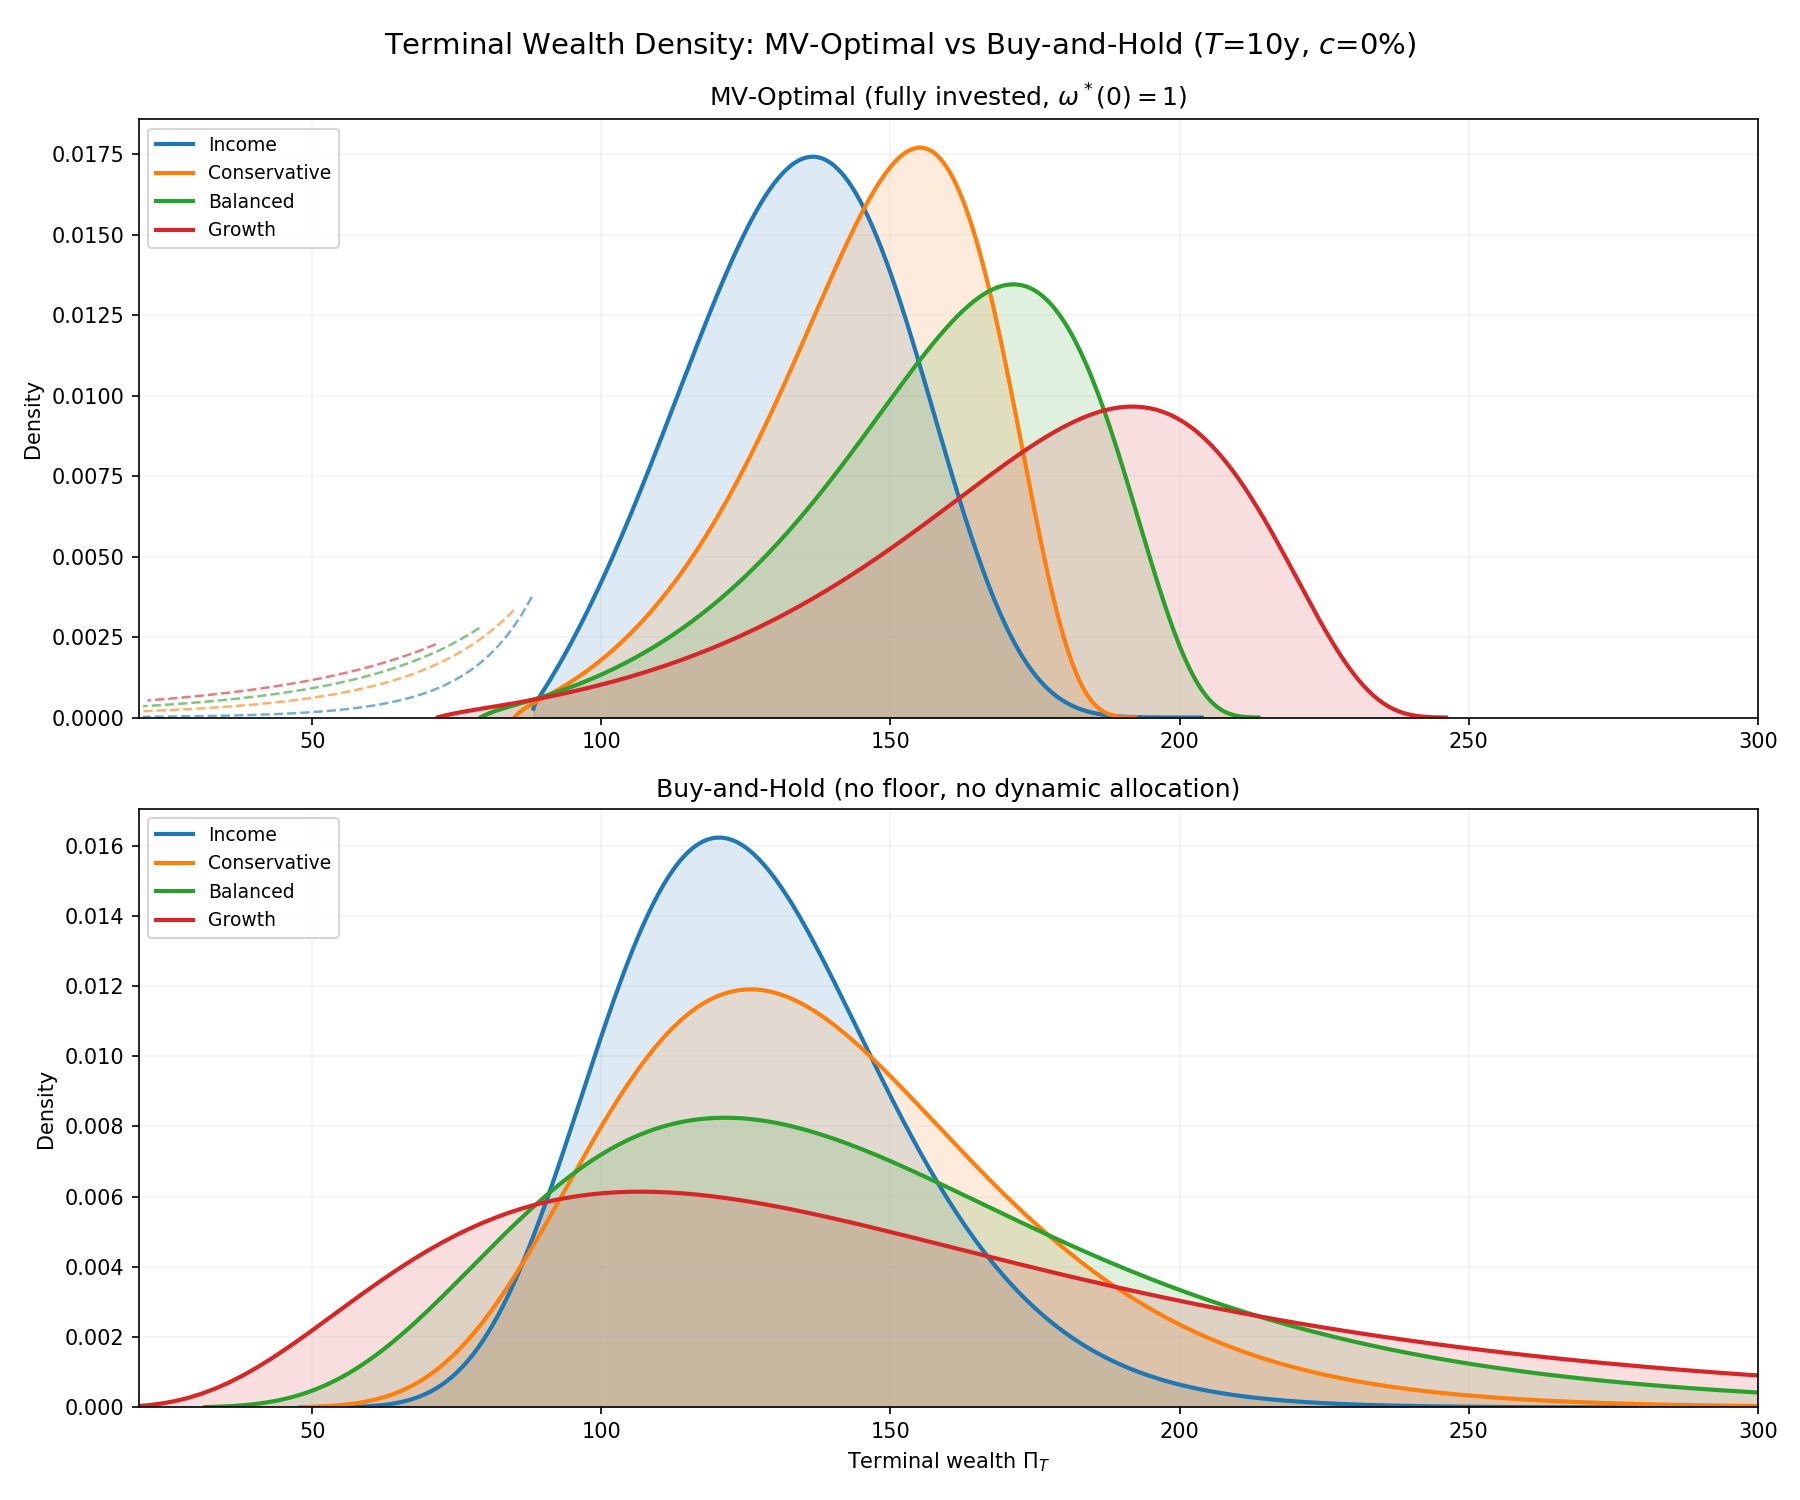
\includegraphics[width=0.825\textwidth]{mandate_density_overlay_c0.png}
\caption{Terminal wealth density for four mandates ($c = 0\%$, 
$\omega^*(0) = 1$, $q_{\mathrm{dd}} = 2$).  Top: MV-optimal strategy 
with floor protection---solid lines show the survived density, bounded 
between $L_T$ and $\Pi^*_T$; dashed lines show the jump-overshoot 
density below the floor (Component~(c) of 
Proposition~\ref{prop:three_components}).  Bottom: buy-and-hold 
benchmark--- densities with wide left tails.  The MV 
strategy concentrates probability mass near the target at the cost 
of capped upside.}
\label{fig:mandate_density_c0}
\end{figure}


Figure~\ref{fig:mandate_comparison} validates the analytical Laplace 
framework against Monte Carlo simulation for the conservative and 
balanced mandates, confirming the accuracy of the constant-coefficient 
approximation (Theorem~\ref{thm:flat_barrier}).

\begin{figure}[H]
\centering
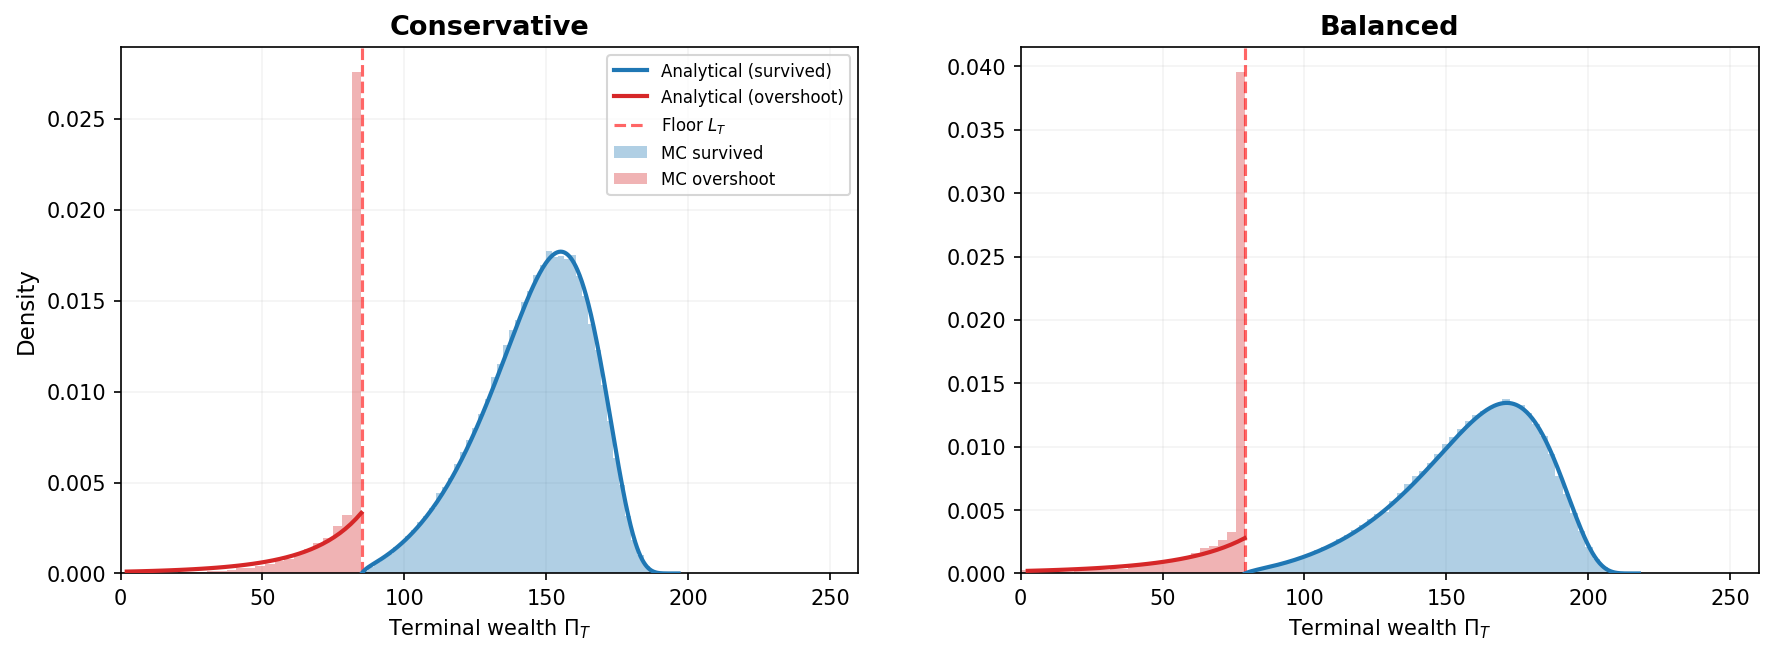
\includegraphics[width=0.825\textwidth]{mandate_comparison.png}
\caption{Analytical survived density (blue) and overshoot density (red) 
overlaid on 200{,}000-path MC histograms (shaded) for conservative and 
balanced mandates ($c = 0\%$, $\omega^*(0) = 1$, $q_{\mathrm{dd}} = 2$). 
Parameters match Table~\ref{tab:mandates}. The $<1$\,pp gap between 
analytical and MC survival probabilities validates the constant-coefficient 
approximation of Theorem~\ref{thm:flat_barrier}.}
\label{fig:mandate_comparison}
\end{figure}




%% ============================================================================
%% SECTION 9: INVESTMENT OPPORTUNITY SET
%% ============================================================================
\section{Investor Profile Construction}\label{sec:opportunity}


\subsection{The inverse problem}\label{sec:inverse}

The mandate analysis of Section~\ref{sec:numerics} fixes the bond weight 
$w$ and computes the terminal wealth distribution $F_w$ analytically. The 
inverse problem asks: given a target terminal wealth profile, which $w$ 
achieves it?

For asset class $j$ with model parameters $\Theta_j$ and policy parameter 
$\pi_j$, the stopped wealth process generates a terminal wealth 
distribution $F_j(\cdot \mid \pi_j; \Theta_j)$. The mixture CDF for 
portfolio weights $\bm{\omega} \in \Delta^{M-1}$ is
\begin{equation}\label{eq:mixture}
F_{\mathrm{mix}}(\cdot \mid \bm{\omega}, \pi) 
= \sum_{j=1}^M \omega_j\, F_j(\cdot \mid \pi_j).
\end{equation}

\begin{proposition}[Achievable distributions]\label{prop:achievable}
For $M \geq 3$ asset classes with distinct effective volatilities, the 
mixture family $\{F_\omega : \omega \in \Delta^{M-1}\}$ spans a 
continuous $(M-1)$-parameter family of terminal wealth distributions 
whose first two moments cover the convex hull of the component moments. 
For $M \to \infty$ (e.g., by subdividing the bond weight 
curve~\eqref{eq:weight_curve}), the family is dense in the Wasserstein-1 
topology over distributions on $(0, \Pi^*_{T,\max}]$ with finite first 
moment.
\end{proposition}

\begin{proof}
See Appendix~\ref{app:density_proof}.
\end{proof}

Proposition~\ref{prop:achievable} guarantees that the family of achievable 
distributions is rich enough to approximate any target. The weight 
parameterisation~\eqref{eq:weight_curve} reduces the simplex $\Delta^{M-1}$ 
to a one-parameter curve indexed by bond weight $w$, and the monotonicity 
of the implied return (Proposition~\ref{prop:r_impl_monotone} below) 
further reduces the investor's decision to selecting a scalar 
$r^*_{\mathrm{impl}}$.


\subsection{Two-step framework}\label{sec:two_step}

\subsubsection{Step 1: Advisor specification}\label{sec:advisor_spec}

The advisor specifies four parameters that, together with the capital 
market assumptions of Table~\ref{tab:params}, determine the investment 
opportunity set as a function of the single free variable $w \in [0, 1]$:
\begin{enumerate}[leftmargin=2em]
\item \textbf{Initial risky allocation} $\omega_0 \in [0.5, 1.5]$: the 
fraction of wealth in the risky portfolio at inception. Default 
$\omega_0 = 1$ (fully invested).
\item \textbf{Consumption rate} $c \in [0\%, 5\%]$: proportional annual 
withdrawal, determining the hurdle rate $r_h = \max(r, c)$ and floor 
growth rate $r_c = r_h - c$.
\item \textbf{Equity--PE split} $g \in [0, 1]$: equity share within the 
risky portfolio, as in~\eqref{eq:weight_curve}. Default $g = 2/3$.
\item \textbf{Drawdown scale} $q_{\mathrm{dd}} \in [1, 3]$: the floor 
is calibrated via~\eqref{eq:k_from_x25}. Default $q_{\mathrm{dd}} = 2$ 
(two-sigma protection).
\end{enumerate}

The equity--PE split fixes a risky composite $R$ with regime parameters 
$(\bar{\mu}^{[i]}_R, \sigma^{[i]}_R, \eta^{[i]}_R)$ independent of $w$. 
Portfolio construction then reduces to a two-asset problem---bonds $B$ 
vs risky composite $R$---with
\begin{equation}\label{eq:two_asset}
\bar{\mu}^{[i]}_{\mathrm{port}}(w) = w\,\bar{\mu}^{[i]}_B + (1-w)\,
\bar{\mu}^{[i]}_R, \quad
\sigma^{[i]}_{\mathrm{port}}(w) = \sqrt{w^2(\sigma^{[i]}_B)^2 
+ 2w(1-w)\rho_{BR}\sigma^{[i]}_B\sigma^{[i]}_R 
+ (1-w)^2(\sigma^{[i]}_R)^2}.
\end{equation}
The crash jump $\eta^{[i]}_{\mathrm{port}}(w)$ is mean-matched 
via~\eqref{eq:eta_port}. For each $w$, the full-investment 
constraint~\eqref{eq:omega_0} pins the Lagrange multiplier $\ell(w)$, the 
drawdown scale determines $k(w)$ via~\eqref{eq:k_from_x25}, and the 
Laplace framework produces $F_w$ with all its moments---approximately one 
second per evaluation on a standard laptop, no numerical optimisation required.

The MV-optimal allocation at inception is 
(Corollary~\ref{cor:optimal_policy}):
\begin{equation}\label{eq:omega_0}
\omega^*(0) = |\omega^*_a| \cdot \left(\frac{\Pi^*(0)}{\Pi_0} 
- 1\right).
\end{equation}
Setting $\omega^*(0) = \omega_0$ gives the target constraint:
\begin{equation}\label{eq:pi_star_0}
\Pi^*(0) = \Pi_0 \left(1 + \frac{\omega_0}{|\omega^*_a(w)|}\right),
\end{equation}
which uniquely determines $\ell(w)$ and hence the growth target 
$g(w) = \frac{1}{T}\ln(\Pi^*_T(w)/\Pi_0)$. Under the full-investment 
constraint, $g$ is an output---not an investor input.

The implied return is the annualised log-growth of expected terminal 
wealth:
\begin{equation}\label{eq:r_impl}
r_{\mathrm{impl}}(w) := \frac{1}{T} \ln \frac{\E[\Pi_T(w)]}{\Pi_0},
\end{equation}
where $\E[\Pi_T(w)]$ is computed from~\eqref{eq:E_Pi}.

\begin{proposition}[Monotonicity of implied return]%
\label{prop:r_impl_monotone}
The implied return $r_{\mathrm{impl}}(w)$ is monotonically decreasing 
in $w$ (increasing in risky allocation $1-w$), provided 
$c < \bar{\mu}_{\mathrm{stat}}(w)$ for all $w$ in the feasible range.
\end{proposition}

The monotonicity follows because $\E[\Pi_T]$ is driven primarily by the 
stationary portfolio return, which increases as the allocation shifts from 
bonds to equity and PE. The floor protection cost also increases with risk, 
but this effect is second order. A portfolio is deemed feasible if 
$r_{\mathrm{impl}}(w) \geq 0$.


\subsubsection{Step 2: Investor selection}\label{sec:client_selection}

The output of Step~1 is the investment opportunity set: $r_{\mathrm{impl}}(w)$ 
together with $F_w$ at each point. The investor selects 
$r^*_{\mathrm{impl}}$, which by 
Proposition~\ref{prop:r_impl_monotone} uniquely determines:
\begin{equation}\label{eq:client_selection}
w^* = r_{\mathrm{impl}}^{-1}(r^*_{\mathrm{impl}}) \quad 
\Longrightarrow \quad
\begin{cases}
\text{Allocation: } w^*_{\mathrm{bd}} / w^*_{\mathrm{eq}} / 
  w^*_{\mathrm{pe}} \text{ via \eqref{eq:weight_curve}}, \\
\text{Floor: } L_0(w^*) \text{ via \eqref{eq:k_from_x25}}, \\
\text{Growth target: } g(w^*) \text{ via \eqref{eq:pi_star_0}}, \\
\text{Distribution: } F_{w^*} \text{ (full CDF from Laplace framework)}.
\end{cases}
\end{equation}

The growth target $g$ is the MV ``ceiling,'' not a return promise. The 
actual expected return is $r_{\mathrm{impl}} \ll g$: for example, the 
growth mandate has $g = 9.3\%$ but $r_{\mathrm{impl}} = 3.7\%$ 
(Table~\ref{tab:mandates}). From~\eqref{eq:E_Pi}:
\begin{equation}\label{eq:gap_decomposition}
\Pi^*_T - \E[\Pi_T] = B_T\!\left(\widetilde{Q}(1) 
+ \widetilde{\Ov}(1)\right) + (\Pi^*_T - L_T)\, F,
\end{equation}
where the three terms quantify the dispersion of survived paths below 
$\Pi^*_T$, the loss from overshoot paths, and the loss from floor-stopped 
paths. In annualised terms, $g - r_{\mathrm{impl}}$ is the implicit 
premium paid for floor protection.


\subsection{Opportunity set illustrations}\label{sec:opp_numerics}

We illustrate the opportunity set for two consumption scenarios: 
$c = 0\%$ (pure accumulation) and $c = 2.5\%$ (income mandate), both 
with $\omega_0 = 1$, $g = 2/3$, $q_{\mathrm{dd}} = 2$, and the asset 
parameters of Table~\ref{tab:params}. Figures~\ref{fig:opp_c0} and~\ref{fig:opp_c25} show the investment 
opportunity set for $c = 0\%$ and $c = 2.5\%$, respectively. Without 
consumption, $r_{\mathrm{impl}}$ ranges from $2.4\%$ (100\% bonds) to 
$3.7\%$ (0\% bonds), and all portfolios are feasible. With $c = 2.5\%$, 
the curve shifts down by approximately $2\%$: the 100\% bond portfolio 
becomes capital-destructive ($r_{\mathrm{impl}} < 0$, survival $25\%$), 
and the feasible region starts at roughly $w = 90\%$. The CDF panels 
show how riskier mandates widen the distribution while lowering the 
floor.


\begin{figure}[H]
\centering

\includegraphics[width=0.775\textwidth]{opportunity_set_c0.png}
\caption{Investment opportunity set, $c = 0\%$. Top left: 
$r_{\mathrm{impl}}$ increases monotonically from $2.4\%$ (100\% bonds) 
to $3.7\%$ (0\% bonds). Top right: efficient frontier in 
$(\sigma_{\mathrm{unc}}, r_{\mathrm{impl}})$ space. Bottom left: CDFs 
for income, conservative, balanced, and growth mandates. Bottom right: 
terminal wealth quantiles with floor $L_T$ (red dashed).}
\label{fig:opp_c0}
\end{figure}
\begin{figure}[H]
\centering

\includegraphics[width=0.775\textwidth]{opportunity_set_c25.png}
\caption{Investment opportunity set, $c = 2.5\%$. Consumption reduces 
$r_{\mathrm{impl}}$ by approximately $2\%$: the range is $-0.3\%$ to 
$1.3\%$. The 100\% bond portfolio is capital-destructive 
($r_{\mathrm{impl}} < 0$, survival $25\%$); the feasible range starts 
at approximately $w = 90\%$.}
\label{fig:opp_c25}
\end{figure}



\subsection{Dynamic allocation}\label{sec:dynamic_alloc}

The MV-optimal policy~\eqref{eq:optimal_w} produces an endogenous 
de-risking glide path: as expected wealth grows toward $\Pi^*(t)$, the 
funding ratio decreases and the allocation moderates---analogous to a 
target-date fund, but derived from the optimisation rather than imposed.

The dollar risky exposure at time $t$, conditional on survival, is
\begin{equation}\label{eq:R_t_def}
R_t := \omega^*(t) \cdot \Pi_t \cdot \ind_{\tau_L > t} 
= |\omega^*_a| \cdot B(t) \cdot e^{-X_t} \cdot \ind_{\tau_L > t},
\end{equation}
where $B(t) = \Pi^*(t) - L_t$. Its first two moments involve the tilted 
survival:
\begin{align}
\E[R_t] &= |\omega^*_a| \cdot B(t) \cdot \widetilde{Q}(t, 1), 
  \label{eq:E_Rt}\\
\Var[R_t] &= |\omega^*_a|^2 \cdot B(t)^2 \cdot 
  \bigl[\widetilde{Q}(t, 2) - \widetilde{Q}(t, 1)^2\bigr].
  \label{eq:Var_Rt}
\end{align}
The expected wealth-weighted allocation and its uncertainty band are
\begin{equation}\label{eq:omega_band}
\bar{\omega}(t) := \frac{\E[R_t]}{\E[\Pi_t]}, \qquad
\bar{\omega}(t) \pm \frac{\mathrm{Std}[R_t]}{\E[\Pi_t]},
\end{equation}
where $\E[\Pi_t]$ is computed from~\eqref{eq:E_Pi_t}. Both numerator 
and denominator are fully analytical via Laplace inversion at each $t$.

The allocation $\bar{\omega}(t)$ decreases over time from two sources: 
funding ratio convergence (the gap $Z_t = \Pi^*(t) - \Pi_t$ shrinks 
relative to wealth) and survival attrition (stopped paths contribute 
zero exposure to the numerator but $L_t$ to the denominator 
of~\eqref{eq:omega_band}).

The de-risking rate depends on the consumption gap $\max(0, c - r)$, not 
on $c$ or $r$ individually. When $c > r$, the persistent wealth drain 
pushes paths toward the floor, increasing stopping probability and 
accelerating de-risking. For the balanced mandate, the $0.5\%$ excess 
withdrawal ($c = 2.5\%$, $r = 2\%$) reduces survival from $79\%$ to 
$60\%$ over $T = 10$ years.



Figure~\ref{fig:risky_allocation} shows the expected risky allocation 
$\bar{\omega}(t)$ with $\pm 1\sigma$ bands for all four mandates at 
$c = 0\%$. All start fully invested and de-risk endogenously: the 
growth mandate falls from $100\%$ to $37\%$ over 10 years, while the 
income mandate maintains the highest allocation beyond $t \approx 1$y 
--- an ordering inversion where the most aggressive mandate de-risks 
fastest because it approaches its target most quickly. The $\pm 1\sigma$ 
band width converges to approximately $60$pp across mandates, driven 
by the binary survived/stopped distinction at longer horizons.


\begin{figure}[H]
\centering

\includegraphics[width=0.825\textwidth]{risky_allocation_subplots_c0.png}
\caption{Expected risky allocation $\bar{\omega}(t) \pm 
\mathrm{Std}[R_t]/\E[\Pi_t]$ for four mandates ($c = 0\%$, 
$\omega_0 = 1$). All mandates start fully invested and de-risk 
endogenously. The growth mandate de-risks fastest (from 100\% to 37\%) 
because it approaches its target most quickly; the income mandate 
maintains the highest allocation at all horizons beyond $t \approx 1$y. 
The $\pm 1\sigma$ band width converges to approximately 60pp across 
mandates, reflecting the dominance of the survived/stopped binary 
distinction at longer horizons.}
\label{fig:risky_allocation}
\end{figure}

A notable property is the ordering inversion: the most aggressive mandate 
de-risks the fastest. In the MV framework, de-risking is proportional to 
the speed at which wealth approaches the target, and aggressive mandates 
close the funding gap faster in expectation.




\section{Conclusion}\label{sec:conclusion}

We have developed a framework for dynamic mean--variance portfolio allocation under regime-switching jump-diffusions with absorbing wealth floors. The MV value function admits a regime-conditional quadratic form whose coupled nonlinear Riccati equations have a unique global solution (Theorem~\ref{thm:riccati_existence}), and the optimal policy retains the Merton--Lipton structure---a regime-dependent Merton ratio modulated by a goal-seeking funding ratio (Corollary~\ref{cor:optimal_policy}).  A Laplace transform framework (Theorem~\ref{thm:char_poly}) provides semi-analytical formulas for survival probabilities, first-passage densities, and conditional moments of the stopped wealth. The stopped wealth process decomposes into three components: survived paths, floor atoms, and jump overshoots (Proposition~\ref{prop:three_components}).   We apply analytical moment formulas, a hurdle rate mechanism $r_h = \max(r,c)$ for consumption, and the Wasserstein-1 density of achievable distributions (Proposition~\ref{prop:achievable}) together to support a two-step construction of investor's wealth policy. This policy maps investor's view on desired return and shape of wealth distribution to a one-parameter family of portfolios with analytically computed wealth distributions, floor protection costs, and endogenous de-risking glide paths---all without Monte Carlo simulation. The mathematical machinery connects three previously separate literatures: dynamic MV allocation \citep{ZhouLi2000,Lipton2001,ZhouYin2003,BieleckiJinPliskaZhou2005,ContTankov2009,ShiXu2025}, barrier option pricing under jump-diffusions \citep{Lipton2001assets,KouWang2003,Sepp2004,BoyarchenkoLevendorskii2012}, and goal-based wealth management \citep{DasEtAl2010,SharpeTinkGoldstein2000}.


Future work includes time-consistent formulations, extension to $N > 2$ regimes (yielding characteristic polynomials of order $3N$), regime filtering with blended allocation policies. Further, our analytical Laplace framework can be coupled with reinforcement learning approaches for path-dependent extensions incorporating portfolio constraints such as no-shorting, leverage limits, and transaction costs, building on \citep{DangForsyth2014, WangZhou2020}.


\paragraph{Conflict of Interest.}
The author is employed by LGT Private Banking. The views expressed 
are the author's own and do not represent those of LGT.


\paragraph{Acknowledgments.}
The author thanks The author thanks Mika Kastenholz and Wladimir Lucic for helpful discussions.


\paragraph{Data Availability Statement.}
All data and code supporting the results are available in the 
companion Python package \texttt{GoalBasedAllocation} at 
\url{https://github.com/ArturSepp/GoalBasedAllocation}.





\bibliographystyle{plainnat}
\begin{thebibliography}{99}

\bibitem[Abate and Whitt(1995)]{AbateWhitt1995}
Abate, J. and Whitt, W. (1995). Numerical inversion of Laplace transforms of probability distributions. \textit{ORSA Journal on Computing}, 7(1):36--43.

\bibitem[Basak and Chabakauri(2010)]{BasakChabakauri2010}
Basak, S. and Chabakauri, G. (2010). Dynamic mean--variance asset allocation. \textit{The Review of Financial Studies}, 23(8):2970--3016.

\bibitem[Bielecki et~al.(2005)]{BieleckiJinPliskaZhou2005}
Bielecki, T.R., Jin, H., Pliska, S.R., and Zhou, X.Y. (2005). Continuous-time mean--variance portfolio selection with bankruptcy prohibition. \textit{Mathematical Finance}, 15(2):213--244.

\bibitem[Boyarchenko and Levendorskii(2012)]{BoyarchenkoLevendorskii2012}
Boyarchenko, M. and Levendorskii, S. (2012). Valuation of continuously monitored double barrier options and related securities. \textit{Mathematical Finance}, 22(3):419--448.

\bibitem[Chen et~al.(2008)]{ChenYaoYin2008}
Chen, P., Yang, H., and Yin, G. (2008). Markowitz's mean--variance asset--liability management with regime switching: A continuous-time model. \textit{Insurance: Mathematics and Economics}, 43(3):456--465.

\bibitem[Cont and Tankov(2009)]{ContTankov2009}
Cont, R. and Tankov, P. (2009). Constant proportion portfolio insurance in the presence of jumps in asset prices. \textit{Mathematical Finance}, 19(3):379--401.

\bibitem[Dang and Forsyth(2014)]{DangForsyth2014}
Dang, D.-M. and Forsyth, P.A. (2014). Continuous time mean--variance optimal portfolio allocation 
under jump diffusion: A numerical impulse control approach. \textit{Numerical Methods for Partial 
Differential Equations}, 30(3):664--698.

\bibitem[Das et~al.(2010)]{DasEtAl2010}
Das, S., Markowitz, H., Scheid, J., and Statman, M. (2010). Portfolio optimization with mental accounts. \textit{Journal of Financial and Quantitative Analysis}, 45(2):311--334.

\bibitem[Farkas et~al.(2021)]{FarkasVasiljevic2021}
Farkas, W., Mathys, L., and Vasiljevi\'c, N. (2021). Intra-horizon expected shortfall and risk structure in models with jumps. \textit{Mathematical Finance}, 31(3):772--823.

\bibitem[Feng and Linetsky(2008)]{FengLinetsky2008}
Feng, L. and Linetsky, V. (2008). Pricing discretely monitored barrier options and defaultable bonds in L\'evy process models: A fast Hilbert transform approach. \textit{Mathematical Finance}, 18(3):337--384.

\bibitem[Grossman and Zhou(1993)]{GrossmanZhou1993}
Grossman, S.J. and Zhou, Z. (1993). Optimal investment strategies for controlling drawdowns. \textit{Mathematical Finance}, 3(3):241--276.

\bibitem[Hamilton(1989)]{Hamilton1989}
Hamilton, J.D. (1989). A new approach to the economic analysis of nonstationary time series and the business cycle. \textit{Econometrica}, 57(2):357--384.

\bibitem[Hu et~al.(2022)]{HuShiXu2022}
Hu, Y., Shi, X., and Xu, Z.Q. (2022). Constrained stochastic LQ control with regime switching and application to portfolio selection. \textit{The Annals of Applied Probability}, 32(1):426--460.

\bibitem[Jiang and Pistorius(2008)]{JiangPistorius2008}
Jiang, Z. and Pistorius, M. (2008). On perpetual American put valuation and first-passage in a regime-switching model with jumps. \textit{Finance and Stochastics}, 12(3):331--355.

\bibitem[Kou(2002)]{Kou2002}
Kou, S. (2002). A jump diffusion model for option pricing. \textit{Management Science}, 48(8):1086--1101.

\bibitem[Kou and Wang(2003)]{KouWang2003}
Kou, S. and Wang, H. (2003). First passage times of a jump diffusion process. \textit{Advances in Applied Probability}, 35(2):504--531.

\bibitem[Lindsay(1995)]{LindsayMixtures1995}
Lindsay, B.G. (1995). \textit{Mixture Models: Theory, Geometry and Applications}. IMS Lecture Notes--Monograph Series.

\bibitem[Lipton(2001a)]{Lipton2001}
Lipton, A. (2001a). \textit{Mathematical Methods for Foreign Exchange}. World Scientific.

\bibitem[Lipton(2001b)]{Lipton2001assets}
Lipton, A. (2001b). Assets with jumps. \textit{Risk}, 14(9):149--153.

\bibitem[Lipton and Lopez de Prado (2026)]{LiptonPrado2026}
Lipton, A. and Lopez de Prado, M. Valuing private equity analytically. \textit{Risk}, April 2026:1--7.

\bibitem[Sepp(2004)]{Sepp2004}
Sepp, A. (2004). Analytical pricing of double-barrier options under a double-exponential jump diffusion process. \textit{International Journal of Theoretical and Applied Finance}, 7(2):151--175.

\bibitem[Sepp(2006)]{Sepp2006}
Sepp, A. (2006). Extended CreditGrades model with stochastic volatility and jumps. \textit{Wilmott Magazine}, September:50--62.

\bibitem[Sepp et~al.(2026a)]{SeppOssaKastenholz2026}
Sepp, A., Ossa, I., and Kastenholz, M. (2026). Robust optimization of strategic and tactical asset allocation for multi-asset portfolios. \textit{Journal of Portfolio Management}, 52(4):86--120.

\bibitem[Sepp et~al.(2026b)]{SeppHansenKastenholz2026}
Sepp, A., Hansen, E., and Kastenholz, M. (2026). Capital market assumptions and strategic asset allocation using multi-asset tradable factors. Under revision at the \textit{Journal of Portfolio Management}.

\bibitem[Sepp(2026b)]{SeppGBA2026}
Sepp, A. (2026). GoalBasedAllocation: A Python package for dynamic mean-variance 
portfolio allocation under regime-switching jump-diffusions. Available at 
\url{https://github.com/ArturSepp/GoalBasedAllocation}.


\bibitem[Sharpe et~al.(2000)]{SharpeTinkGoldstein2000}
Sharpe, W.F., Goldstein, D.G., and Blythe, P.W. (2000). The distribution builder: A tool for inferring investor preferences. \textit{Working paper, Stanford University}.

\bibitem[Shi and Xu(2025)]{ShiXu2025}
Shi, X. and Xu, Z.Q. (2025). Optimal mean--variance portfolio selection under regime-switching-induced stock price shocks. \textit{Systems \& Control Letters}, forthcoming.

\bibitem[Siu et~al.(2014)]{SiuEtAl2014}
Siu, C.C., Ladkau, M., Langren\'e, N., and Pham, H. (2014). On the first passage time under regime-switching with jumps. In \textit{Inspired by Finance}, Springer, pp.~387--410.

\bibitem[Sotomayor and Cadenillas(2009)]{SotomayorCadenillas2009}
Sotomayor, L.R. and Cadenillas, A. (2009). Explicit solutions of consumption--investment problems in financial markets with regime switching. \textit{Mathematical Finance}, 19(2):251--279.

\bibitem[Wang and Zhou(2020)]{WangZhou2020}
Wang, H. and Zhou, X.Y. (2020). Continuous-time mean--variance portfolio selection: A reinforcement learning framework. \textit{Mathematical Finance}, 30(4):1273--1308.

\bibitem[Xie(2008)]{Xie2008}
Xie, S. (2008). Continuous-time mean--variance portfolio selection with liability and regime switching. \textit{Insurance: Mathematics and Economics}, 42(3):943--953.

\bibitem[Zhou and Li(2000)]{ZhouLi2000}
Zhou, X.Y. and Li, D. (2000). Continuous-time mean--variance portfolio selection: A stochastic LQ framework. \textit{Applied Mathematics and Optimization}, 42(1):19--33.

\bibitem[Zhou and Yin(2003)]{ZhouYin2003}
Zhou, X.Y. and Yin, G. (2003). Markowitz's mean--variance portfolio selection with regime switching: A continuous-time model. \textit{SIAM Journal on Control and Optimization}, 42(4):1466--1482.

\end{thebibliography}


%% ============================================================================
%% APPENDICES
%% ============================================================================
\begin{appendices}

\section{MV Problem Proofs}\label{app:mv_proofs}

\subsection{Proof of Theorem~\ref{thm:quadratic_ansatz}: Quadratic Ansatz}\label{app:quadratic}

\paragraph{Jump integral computation.}\label{app:jump_integral}

We verify that the jump expectation of a quadratic function remains quadratic. Let $V^{[2]}(\tau, \Pi) = a^{[2]}\Pi^2 + b^{[2]}\Pi + \gamma^{[2]}$ and compute:
\begin{align}
& \E\!\left[V^{[2]}(\tau, \Pi(1+\varpi(e^{J^{[1]}}-1)))\right] \notag \\
&= a^{[2]} \Pi^2 \E[(1+\varpi(e^{J^{[1]}}-1))^2] + b^{[2]} \Pi \E[1+\varpi(e^{J^{[1]}}-1)] + \gamma^{[2]}.
\label{eq:jump_quad_detail}
\end{align}

The required expectations, using \eqref{eq:jump_mgf} with $J^{[1]} \sim -\mathrm{Exp}(1/\eta^{[1]})$:
\begin{align}
\E[e^{J^{[1]}}] &= \frac{1}{1 + \eta^{[1]}}, \quad
\E[e^{2J^{[1]}}] = \frac{1}{1 + 2\eta^{[1]}}, \label{eq:jump_exp_moments} \\
\alpha^{[1]} &= \E[e^{J^{[1]}}-1] = \frac{-\eta^{[1]}}{1+\eta^{[1]}}, \label{eq:alpha1_detail} \\
(\sigma_J^{[1]})^2 &= \E[(e^{J^{[1]}}-1)^2] = \frac{1}{1+2\eta^{[1]}} - \frac{2}{1+\eta^{[1]}} + 1. \label{eq:sigJ1_detail}
\end{align}

Therefore:
\begin{align}
\E[(1+\varpi(e^{J^{[1]}}-1))^2] &= 1 + 2\varpi\alpha^{[1]} + \varpi^2 (\sigma_J^{[1]})^2, \label{eq:E_square} \\
\E[1+\varpi(e^{J^{[1]}}-1)] &= 1 + \varpi\alpha^{[1]}. \label{eq:E_linear}
\end{align}

Substituting into \eqref{eq:jump_quad_detail}:
\begin{equation}
\E[V^{[2]}(\cdot)] = a^{[2]}\Pi^2[1 + 2\varpi\alpha^{[1]} + \varpi^2(\sigma_J^{[1]})^2] + b^{[2]}\Pi[1+\varpi\alpha^{[1]}] + \gamma^{[2]},
\end{equation}
which is indeed quadratic in $\Pi$ and quadratic in $\varpi$. \qed

\paragraph{Drift cancellation.}\label{app:drift_cancel}

The FOC in regime~1, differentiating with respect to $\varpi$:
\begin{align}
0 &= (\mu^{[1]} - r_h)(2a^{[1]}\Pi + b^{[1]})\Pi + 2\varpi(\sigma^{[1]})^2 a^{[1]} \Pi^2 \notag \\
&\quad + \lambda^{[12]}\left[2\alpha^{[1]} a^{[2]} \Pi^2 + \alpha^{[1]} b^{[2]} \Pi + 2\varpi(\sigma_J^{[1]})^2 a^{[2]} \Pi^2\right]. \label{eq:foc_full}
\end{align}

Collecting the terms not involving $\varpi$:
\begin{align}
& (\mu^{[1]} - r_h)(2a^{[1]}\Pi + b^{[1]})\Pi + \lambda^{[12]}\alpha^{[1]}(2a^{[2]}\Pi^2 + b^{[2]}\Pi) \notag \\
&= \left[(\mu^{[1]} - r_h)2a^{[1]} + 2\lambda^{[12]}\alpha^{[1]} a^{[2]}\right]\Pi^2 + \left[(\mu^{[1]}-r_{h})b^{[1]} + \lambda^{[12]}\alpha^{[1]} b^{[2]}\right]\Pi \notag \\
&= 2\tilde{a}^{[1]} \Pi^2 + \tilde{b}^{[1]} \Pi, \label{eq:tilde_collect}
\end{align}
where $\tilde{a}^{[1]}$ and $\tilde{b}^{[1]}$ are defined in \eqref{eq:RS_def}. Using $\bar{\mu}^{[1]} = \mu^{[1]} + \lambda^{[12]}\alpha^{[1]}$:
\begin{align}
\tilde{a}^{[1]} &= (\bar{\mu}^{[1]} - r_h - \lambda^{[12]}\alpha^{[1]})a^{[1]} + \lambda^{[12]}\alpha^{[1]} a^{[2]} = (\bar{\mu}^{[1]}-r_h)a^{[1]} + \lambda^{[12]}\alpha^{[1]}(a^{[2]} - a^{[1]}). \label{eq:tilde_a_expand}
\end{align}
The $\varpi$-coefficient:
\begin{equation}
2\Sigma^{[1]}\Pi^2 = 2\left[(\sigma^{[1]})^2 a^{[1]} + \lambda^{[12]}(\sigma_J^{[1]})^2 a^{[2]}\right]\Pi^2. \label{eq:S_coeff}
\end{equation}

The FOC becomes $2\tilde{a}^{[1]}\Pi + \tilde{b}^{[1]} + 2\varpi \Sigma^{[1]} \Pi = 0$, yielding the optimal $\varpi^{*[1]}$ in \eqref{eq:optimal_w}. \qed


\subsection{Full ODE System}\label{app:full_odes}

After substituting the optimal $\varpi^{*[i]}$ back into the HJB, all $\varpi$-dependent terms combine into the quadratic completion. The terms independent of $\varpi$ yield the regime-switching coupling. Collecting by powers of $\Pi$:

\paragraph{Reduced HJB.}\label{app:reduced_hjb} Define $\varpi^{*[i]}_a := -\tilde{a}^{[i]}/\Sigma^{[i]}$ (the regime-$i$ allocation coefficient). Substituting $\varpi^{*[i]}_t = \varpi^{*[i]}_a + \tilde{b}^{[i]}/(2\Sigma^{[i]}\Pi)$ into the infimum and using the identity $\min_\varpi [\varpi(2R\Pi + B)\Pi + \varpi^2 \Sigma\Pi^2] = -(2R\Pi+B)^2/(4\Sigma)$, we obtain:
\begin{equation}\label{eq:reduced_hjb_full}
\begin{split}
0 = &\;-{a^{[i]}}'(\tau)\Pi^2 - {b^{[i]}}'(\tau)\Pi - {\gamma^{[i]}}'(\tau) + r_c(2a^{[i]}\Pi^2 + b^{[i]}\Pi) \\
&\;- \frac{(\tilde{a}^{[i]})^2}{\Sigma^{[i]}}\Pi^2 - \frac{\tilde{a}^{[i]}\tilde{b}^{[i]}}{\Sigma^{[i]}}\Pi - \frac{(\tilde{b}^{[i]})^2}{4\Sigma^{[i]}} + \lambda^{[i\to j]}\!\left[(a^{[j]} - a^{[i]})\Pi^2 + (b^{[j]}-b^{[i]})\Pi + (\gamma^{[j]}-\gamma^{[i]})\right].
\end{split}
\end{equation}

\paragraph{$\Pi^2$ equations.}\label{app:pi2_eqs}
\begin{align}
{a^{[1]}}' &= (2r_c - \lambda^{[12]})a^{[1]} + \lambda^{[12]} a^{[2]} - \frac{(\tilde{a}^{[1]})^2}{\Sigma^{[1]}}, \label{eq:ode_a1_simple} \\
{a^{[2]}}' &= (2r_c - \lambda^{[21]})a^{[2]} + \lambda^{[21]} a^{[1]} - \frac{(\tilde{a}^{[2]})^2}{\Sigma^{[2]}}, \label{eq:ode_a2_simple}
\end{align}
with $a^{[1]}(0) = a^{[2]}(0) = 1$. The nonlinearity arises because $\tilde{a}^{[i]}$ and $\Sigma^{[i]}$ are functions of $(a^{[1]}, a^{[2]})$.

\paragraph{$\Pi$ equations.}\label{app:pi_eqs}
\begin{align}
{b^{[1]}}' &= (r_c - \lambda^{[12]})b^{[1]} + \lambda^{[12]} b^{[2]} - \frac{\tilde{a}^{[1]} \tilde{b}^{[1]}}{\Sigma^{[1]}}, \label{eq:ode_b1} \\
{b^{[2]}}' &= (r_c - \lambda^{[21]})b^{[2]} + \lambda^{[21]} b^{[1]} - \frac{\tilde{a}^{[2]} \tilde{b}^{[2]}}{\Sigma^{[2]}}, \label{eq:ode_b2}
\end{align}
with $b^{[1]}(0) = b^{[2]}(0) = -\ell$. Linearity in $(b^{[1]}, b^{[2]})$ follows because $\tilde{a}^{[i]}/\Sigma^{[i]} = \varpi^{*[i]}_a$ depends only on $(a^{[1]}, a^{[2]})$, which are already determined. Explicitly, using $\tilde{b}^{[i]} = (\mu^{[i]}-r_h)b^{[i]} + \lambda^{[i\to j]}\alpha^{[i]} b^{[j]}$:
\begin{equation}\label{eq:ode_b_matrix}
\begin{pmatrix} {b^{[1]}}' \\ {b^{[2]}}' \end{pmatrix} = \underbrace{\begin{pmatrix}
r_c - \lambda^{[12]} + \varpi^{*[1]}_a(\mu^{[1]}-r_h) & \lambda^{[12]}(1 + \varpi^{*[1]}_a \alpha^{[1]}) \\
\lambda^{[21]}(1 + \varpi^{*[2]}_a \alpha^{[2]}) & r_c - \lambda^{[21]} + \varpi^{*[2]}_a(\mu^{[2]}-r_h)
\end{pmatrix}}_{\displaystyle =: \mathbf{B}(\tau)} \begin{pmatrix} b^{[1]} \\ b^{[2]} \end{pmatrix}.
\end{equation}

\noindent Derivation. Using $\tilde{a}^{[i]}/\Sigma^{[i]} = -\varpi^{*[i]}_a$ and $\tilde{b}^{[i]} = (\mu^{[i]}-r_h)b^{[i]} + \lambda^{[i\to j]}\alpha^{[i]}b^{[j]}$:
\begin{equation}\label{eq:b_derivation}
-\frac{\tilde{a}^{[i]}\tilde{b}^{[i]}}{\Sigma^{[i]}} = \varpi^{*[i]}_a \tilde{b}^{[i]} = \varpi^{*[i]}_a\!\left[(\mu^{[i]}-r_h)b^{[i]} + \lambda^{[i\to j]}\alpha^{[i]}b^{[j]}\right].
\end{equation}
Adding this to $(r_c-\lambda^{[i\to j]})b^{[i]} + \lambda^{[i\to j]}b^{[j]}$ from the regime-switching coupling, we obtain $\mathbf{B}(\tau)$.

The matrix $\mathbf{B}(\tau)$ admits a natural interpretation. The diagonal entries $r_c - \lambda^{[i\to j]} + \varpi^{*[i]}_a(\mu^{[i]}-r_h)$ combine the cash growth rate, the switching intensity, and the drift effect of the optimal allocation at the $\Pi^2$ level. Since $\varpi^{*[i]}_a < 0$ (shorting at high wealth) and $\mu^{[i]} - r_h > 0$, the allocation reduces the effective growth rate. The off-diagonal entries $\lambda^{[i\to j]}(1 + \varpi^{*[i]}_a\alpha^{[i]})$ represent the switching intensities modulated by the expected jump multiplier $\E[1 + \varpi^{*[i]}_a(e^{J^{[i]}}-1)] = 1 + \varpi^{*[i]}_a\alpha^{[i]}$ under the optimal allocation. Since $\varpi^{*[i]}_a\alpha^{[i]} > 0$ (product of two negatives for regime~1), the effective switching intensity in the $b$-equation exceeds the bare intensity $\lambda^{[i\to j]}$. Since $(a^{[1]}, a^{[2]})$ are already determined, $\mathbf{B}(\tau)$ is a known matrix-valued function and \eqref{eq:ode_b_matrix} is a linear non-autonomous $2 \times 2$ system with unique solution.

\paragraph{$\Pi^0$ equations.}\label{app:pi0_eqs}
\begin{align}
{\gamma^{[1]}}' &= -\lambda^{[12]}\gamma^{[1]} + \lambda^{[12]}\gamma^{[2]} - \frac{(\tilde{b}^{[1]})^2}{4\Sigma^{[1]}}, \label{eq:ode_g1} \\
{\gamma^{[2]}}' &= -\lambda^{[21]}\gamma^{[2]} + \lambda^{[21]}\gamma^{[1]} - \frac{(\tilde{b}^{[2]})^2}{4\Sigma^{[2]}}, \label{eq:ode_g2}
\end{align}
with $\gamma^{[1]}(0) = \gamma^{[2]}(0) = 0$.


\subsection{Proof of Theorem~\ref{thm:riccati_existence}: Riccati Existence}\label{app:riccati_existence}

We prove that the coupled system \eqref{eq:ode_a1_simple}--\eqref{eq:ode_a2_simple} has a unique positive global solution.

\begin{proof}
\textbf{Step~1: Local existence.} The right-hand side of \eqref{eq:ode_a1_simple}--\eqref{eq:ode_a2_simple} is locally Lipschitz in $(a^{[1]}, a^{[2]}) \in (0,\infty)^2$ (the nonlinearity $(\tilde{a}^{[1]})^2/\Sigma^{[1]}$ is a rational function of $a^{[1]}, a^{[2]}$ with denominator bounded away from zero for $a^{[i]} > 0$). By the Picard--Lindel\"of theorem, a unique local solution exists on $[0, T_*)$ for some $T_* > 0$.

\textbf{Step~2: Positivity.} We show $a^{[i]}(\tau) > 0$ for all $\tau \in [0, T_*)$. Note that $(\tilde{a}^{[1]})^2/\Sigma^{[1]} \leq C(a^{[1]} + a^{[2]})$ for some constant $C > 0$ (since $\tilde{a}$ and $S$ are linear combinations of $a^{[i]}$). The linear part $(2r_c - \lambda^{[12]})a^{[1]} + \lambda^{[12]} a^{[2]}$ preserves positivity (the matrix $\begin{psmallmatrix} 2r_c-\lambda^{[12]} & \lambda^{[12]} \\ \lambda^{[21]} & 2r_c-\lambda^{[21]} \end{psmallmatrix}$ has nonneg.\ off-diagonal entries). By comparison with the linear system (dropping the negative $-(\tilde{a})^2/S$ term), $a^{[i]}(\tau) > 0$.

\textbf{Step~3: Upper bound.} Since $(\tilde{a})^2/S \geq 0$, we have $a^{[i]}(\tau) \leq \bar{a}^{[i]}(\tau)$ where $\bar{a}$ solves the linear system without the quadratic term. This linear system has exponential solutions bounded on $[0,T]$.

\textbf{Step~4: Global existence.} Steps~2--3 give $0 < a^{[i]}(\tau) \leq C e^{CT}$ on $[0, T_*)$. The solution cannot blow up in finite time, so $T_* = \infty$.
\end{proof}


\subsection{Proof of Theorem~\ref{thm:verification}: Verification}\label{app:verification}

\begin{proof}
We apply It\^o's formula to $V^{[\chi_t]}(\tau, \Pi_t)$ for $\tau = T - t$. Between transitions:
\begin{equation}
\dd V^{[\chi_t]} = \left(-V^{[\chi_t]}_\tau + r_c\Pi V^{[\chi_t]}_\Pi + \varpi(\mu^{[\chi_t]}-r_h)\Pi V^{[\chi_t]}_\Pi + \tfrac{1}{2}\varpi^2(\sigma^{[\chi_t]})^2\Pi^2 V^{[\chi_t]}_{\Pi\Pi}\right)\dd t + (\ldots)\dd W_t.
\end{equation}

At regime transition from $i$ to $j$ with jump factor $(1+\varpi(e^{J^{[i]}}-1))$:
\begin{equation}
\Delta V = V^{[j]}(\tau, \Pi(1+\varpi(e^{J^{[i]}}-1))) - V^{[i]}(\tau, \Pi).
\end{equation}

The compensated process $M_t := V^{[\chi_t]}(T-t, \Pi_t) - V^{[\chi_0]}(T, \Pi_0) - \int_0^t (\ldots) \dd s$ is a local martingale. For the optimal $\varpi^*$, the drift terms cancel by construction of the ODE system, so $V^{[\chi_t]}(T-t, \Pi_t)$ is a (local) martingale under $\varpi^*$.

To upgrade to a true martingale, we verify the integrability condition $\E[\sup_{t \leq T} |V^{[\chi_t]}(T-t, \Pi_t)|] < \infty$, which follows from the quadratic structure and the boundedness of $a^{[i]}(\tau)$ (Theorem~\ref{thm:riccati_existence}).

For any admissible $\varpi$, the drift is $\geq 0$ (since $\varpi^*$ 
achieves the infimum), so $V^{[\chi_t]}(T-t, \Pi_t)$ is a submartingale. 
Under $\varpi^*$ the drift vanishes and $V$ is a martingale, giving:
\begin{equation}
\E_{\varpi^*}[\Pi_T^2 - \ell \Pi_T] = V^{[\chi_0]}(T, \Pi_0) 
\leq \E_{\varpi}[\Pi_T^2 - \ell \Pi_T] \quad 
\text{for all admissible } \varpi,
\end{equation}
confirming optimality.


\paragraph{Admissibility.}\label{app:admissibility}

We verify that the optimal policy $\varpi^{*[\chi_t]}_t$ from \eqref{eq:optimal_w} belongs to the admissible set $\mathcal{A}$, \ie\ $\varpi^*$ is $\F_t$-adapted and $\E[\Pi_T^2] < \infty$.

Adaptedness is immediate: $\varpi^{*[i]}_t = |\omega^*_a(\tau)| \cdot (\Pi^{*[i]}(t)/\Pi_t - 1)$ depends on $\Pi_t$ (observed), $\chi_t$ (observed), and deterministic functions of $\tau = T - t$.

For square-integrability, we establish $\E[\sup_{t \leq T} \Pi_t^2] < \infty$.  The wealth process satisfies $\Pi_t = \Pi^{*[\chi_t]}(t) - Z_t$ where $Z_t > 0$ is the gap.  Since $\Pi^{*[i]}(t)$ is bounded on $[0, T]$ (it equals $-b^{[i]}(T-t)/(2a^{[i]}(T-t))$ with bounded $a, b$), it suffices to show $\E[\sup_{t \leq T} Z_t^2] < \infty$.

Between transitions, the gap satisfies $\dd Z/Z = \mu_Z^{[i]}\,\dd t + \sigma_Z^{[i]}\,\dd W$ with bounded coefficients $\mu_Z^{[i]}$, $\sigma_Z^{[i]}$ (since $|\omega^*_a|$ is bounded and continuous in $\tau$).  At transition $i \to j$, the multiplicative jump factor is $1 + |\omega^*_a|(1 - e^{J^{[i]}})$.  For crash jumps ($J^{[1]} < 0$), this factor lies in $(0, 1 + |\omega^*_a|)$ and satisfies
\begin{equation}\label{eq:jump_sq_integ}
\E[(1 + |\omega^*_a|(1 - e^{J^{[1]}}))^2] = 1 + 2|\omega^*_a|\alpha^{[1]} + |\omega^*_a|^2 (\sigma_J^{[1]})^2 < \infty,
\end{equation}
since $\alpha^{[1]}$ and $(\sigma_J^{[1]})^2$ are finite (Assumption~\ref{ass:params}).  For recovery jumps ($J^{[2]} > 0$), the factor is $1 + |\omega^*_a|(e^{J^{[2]}} - 1) > 1$, and
\begin{equation}\label{eq:jump_sq_integ2}
\E[(1 + |\omega^*_a|(e^{J^{[2]}} - 1))^2] = 1 + 2|\omega^*_a|\alpha^{[2]} + |\omega^*_a|^2 (\sigma_J^{[2]})^2 < \infty,
\end{equation}
using $\eta^{[2]} < 1/2$ (Assumption~\ref{ass:params}), which ensures $\E[e^{2J^{[2]}}] = 1/(1 - 2\eta^{[2]}) < \infty$.

By the Burkholder--Davis--Gundy inequality for the continuous martingale part and the finite second moment of the jump factors, we obtain
\[
\E\!\left[\sup_{t \leq T} Z_t^2\right] \leq C(T)\, Z_0^2 \cdot \prod_{n=1}^{N_T} \E\!\left[\text{jump factor}_n^2\right],
\]
where $N_T$ is the (Poisson-distributed) number of transitions in $[0, T]$, and $C(T)$ is a constant depending on $T$, $\mu_Z$, $\sigma_Z$.  Since $\E[N_T] < \infty$ and each jump factor has finite second moment, the product has finite expectation (by independence of jump sizes), giving $\E[\sup_{t \leq T} Z_t^2] < \infty$.

Therefore $\E[\Pi_T^2] \leq 2(\Pi^{*}_{\max})^2 + 2\E[Z_T^2] < \infty$, confirming $\varpi^* \in \mathcal{A}$.  The upgrade from local to true martingale in the proof of Theorem~\ref{thm:verification} follows from this uniform integrability. \qed

The efficient frontier follows from computing $\Var[\Pi_T] = V^{[i]}(T,\Pi_0) + \ell^2/4$ (with growth rate $r_c$) and optimising over $\ell$.
\end{proof}




\subsection{Moments of buy-and-hold strategy under regime-switching model.}\label{app:bh_moments}

\begin{proposition}[Buy-and-hold moments under RS-JD]\label{prop:bh_moments}
The $n$-th moment $M_n^{[i]}(\tau) = \E[\Pi_T^n \mid \chi_0 = i]$ of the 
buy-and-hold terminal wealth satisfies the $2 \times 2$ linear ODE
\begin{equation}\label{eq:bh_moment_ode}
\frac{\dd}{\dd\tau} \begin{pmatrix} h_n^{[1]} \\ h_n^{[2]} \end{pmatrix}
= \mathbf{A}_n \begin{pmatrix} h_n^{[1]} \\ h_n^{[2]} \end{pmatrix}, 
\qquad h_n^{[1]}(0) = h_n^{[2]}(0) = 1,
\end{equation}
where $M_n^{[i]} = \Pi_0^n\, h_n^{[i]}(T)$ and the matrix entries are
\begin{equation}\label{eq:An_matrix}
\mathbf{A}_n = \begin{pmatrix}
n\mu^{[1]} + \tfrac{n(n-1)}{2}(\sigma^{[1]})^2 - \lambda^{[12]} 
  & \lambda^{[12]} \E[e^{nJ^{[1]}}] \\
\lambda^{[21]} \E[e^{nJ^{[2]}}] 
  & n\mu^{[2]} + \tfrac{n(n-1)}{2}(\sigma^{[2]})^2 - \lambda^{[21]}
\end{pmatrix},
\end{equation}
with $\E[e^{nJ^{[1]}}] = 1/(1+n\eta^{[1]})$ and 
$\E[e^{nJ^{[2]}}] = 1/(1-n\eta^{[2]})$.
The solution is $h_n(T) = e^{\mathbf{A}_n T} \cdot \mathbf{1}$.
The unconditional moments use stationary weights 
$M_n = p_1 M_n^{[1]} + p_2 M_n^{[2]}$.
\end{proposition}


\section{Laplace Framework Proofs}\label{app:laplace_proofs}

\subsection{Characteristic Polynomial Coefficients}\label{app:poly_coeffs}

The coefficients of the sixth-order polynomial $\mathcal{P}(\psi) = \sum_{k=0}^6 w_k \psi^k$ from \eqref{eq:poly6} are obtained by expanding $G^{[1]}(\psi)G^{[2]}(\psi) - \lambda^{[12]}\lambda^{[21]}$ using the forward definitions \eqref{eq:G_def}. Writing $s^{[i]} := \tfrac{1}{2}(\sigma^{[i]})^2$ and $q^{[i]} := \lambda^{[i\to j]} + p$:
\begin{align}
w_0 &= q^{[1]}q^{[2]} - \lambda^{[12]}\lambda^{[21]} = p(\lambda^{[12]}+\lambda^{[21]}+p), \notag \\
w_1 &= (\eta^{[2]}-\eta^{[1]})q^{[1]}q^{[2]} + \nu^{[1]}q^{[2]} + \nu^{[2]}q^{[1]}, \notag \\
w_2 &= -s^{[1]}q^{[2]} - s^{[2]}q^{[1]} - \eta^{[1]}\eta^{[2]}q^{[1]}q^{[2]} + (\eta^{[2]}-\eta^{[1]})(\nu^{[1]}q^{[2]}+\nu^{[2]}q^{[1]}) + \nu^{[1]}\nu^{[2]}, \notag \\
w_3 &= (\eta^{[1]}-\eta^{[2]})(s^{[1]}q^{[2]}+s^{[2]}q^{[1]}) - s^{[1]}\nu^{[2]} - s^{[2]}\nu^{[1]} \notag \\
&\quad - \eta^{[1]}\eta^{[2]}(\nu^{[1]}q^{[2]}+\nu^{[2]}q^{[1]}) + (\eta^{[2]}-\eta^{[1]})\nu^{[1]}\nu^{[2]}, \notag \\
w_4 &= s^{[1]}s^{[2]} + (s^{[1]}q^{[2]}+s^{[2]}q^{[1]})\eta^{[1]}\eta^{[2]} + (s^{[1]}\nu^{[2]}+s^{[2]}\nu^{[1]})(\eta^{[1]}-\eta^{[2]}) - \eta^{[1]}\eta^{[2]}\nu^{[1]}\nu^{[2]}, \notag \\
w_5 &= (s^{[1]}\nu^{[2]}+s^{[2]}\nu^{[1]})\eta^{[1]}\eta^{[2]} + s^{[1]}s^{[2]}(\eta^{[2]}-\eta^{[1]}), \notag \\
w_6 &= -s^{[1]}s^{[2]}\eta^{[1]}\eta^{[2]}. \label{eq:w_coeffs}
\end{align}
Since $w_6 < 0$ and $w_0 > 0$ for $p > 0$, the polynomial changes sign, confirming the existence of real roots. The no-jump limit $\eta^{[1]}, \eta^{[2]} \to 0$ reduces to the quartic $w_0 + w_1\psi + w_2\psi^2 + w_3\psi^3 + s^{[1]}s^{[2]}\psi^4 = 0$.


\subsection{Proof of Theorem~\ref{thm:char_poly}: Characteristic Polynomial}\label{app:char_poly}

\begin{proof}
We substitute the exponential ansatz $\hat{A}^{[1]} = a_k e^{\psi_k X}$, $\hat{A}^{[2]} = b_k e^{\psi_k X}$ into the Laplace-transformed forward OIDE \eqref{eq:forward_generator}. The recovery jump integral (regime~2 to regime~1 coupling) yields:
\begin{align}
\lambda^{[21]}\!\int_0^{\infty} b_k e^{\psi_k(X-J)} f^{[2]}(J) \dd J &= \lambda^{[21]} b_k e^{\psi_k X} \cdot \frac{1}{1 + \eta^{[2]}\psi_k}, \quad \text{for } \psi_k > -1/\eta^{[2]}.
\end{align}

The crash jump integral (regime~1 to regime~2 coupling) yields:
\begin{align}
\lambda^{[12]}\!\int_{-\infty}^0 a_k e^{\psi_k(X-J)} f^{[1]}(J) \dd J &= \lambda^{[12]} a_k e^{\psi_k X} \cdot \frac{1}{1 - \eta^{[1]}\psi_k}, \quad \text{for } \psi_k < 1/\eta^{[1]}.
\end{align}

Substituting into the forward OIDE and cancelling $e^{\psi_k X}$:
\begin{align}
\left[\tfrac{1}{2}(\sigma^{[1]})^2\psi_k^2 - \nu^{[1]}\psi_k - (\lambda^{[12]}+p)\right] a_k + \lambda^{[21]} \frac{b_k}{1+\eta^{[2]}\psi_k} &= 0, \label{eq:char_sys1} \\
\left[\tfrac{1}{2}(\sigma^{[2]})^2\psi_k^2 - \nu^{[2]}\psi_k - (\lambda^{[21]}+p)\right] b_k + \lambda^{[12]} \frac{a_k}{1-\eta^{[1]}\psi_k} &= 0. \label{eq:char_sys2}
\end{align}

Define $Q^{[i]}(\psi) := -\tfrac{1}{2}(\sigma^{[i]})^2\psi^2 + \nu^{[i]}\psi + q^{[i]}$ with $q^{[i]} = \lambda^{[i\to j]} + p$, so the bracket in \eqref{eq:char_sys1} is $-Q^{[1]}(\psi_k)$. Multiply \eqref{eq:char_sys1} by $(1+\eta^{[2]}\psi_k)$ and \eqref{eq:char_sys2} by $(1-\eta^{[1]}\psi_k)$:
\begin{align}
-Q^{[1]}(\psi_k)(1+\eta^{[2]}\psi_k) \, a_k + \lambda^{[21]} b_k &= 0, \label{eq:Gb_sys1} \\
-Q^{[2]}(\psi_k)(1-\eta^{[1]}\psi_k) \, b_k + \lambda^{[12]} a_k &= 0. \label{eq:Gb_sys2}
\end{align}
Recalling $G^{[1]}(\psi) = (1-\eta^{[1]}\psi)Q^{[1]}(\psi)$ and $G^{[2]}(\psi) = (1+\eta^{[2]}\psi)Q^{[2]}(\psi)$ from \eqref{eq:G_def}, a non-trivial solution $(a_k, b_k) \neq (0,0)$ exists iff $\det = 0$:
\begin{equation}
Q^{[1]}(\psi_k)(1+\eta^{[2]}\psi_k) \cdot Q^{[2]}(\psi_k)(1-\eta^{[1]}\psi_k) = \lambda^{[12]}\lambda^{[21]},
\end{equation}
which is $G^{[1]}(\psi_k) G^{[2]}(\psi_k) = \lambda^{[12]}\lambda^{[21]}$, confirming \eqref{eq:char_poly}.

Since $G^{[1]}$ and $G^{[2]}$ are each cubic, $\mathcal{P}(\psi) = G^{[1]}G^{[2]} - \lambda^{[12]}\lambda^{[21]}$ is degree~6. Expanding yields \eqref{eq:w_coeffs}.

\medskip\noindent\textbf{Coupling ratio.} From \eqref{eq:Gb_sys1}, the physical coupling is $b_k/a_k = Q^{[1]}(\psi_k)(1+\eta^{[2]}\psi_k) / \lambda^{[21]} =: \beta_k$ as stated in \eqref{eq:physical_coupling}. For the $6\times 6$ matching system (Appendix~\ref{app:6x6_system}) and the $3 \times 3$ barrier system (Appendix~\ref{app:bounded_proof}), we define the system coupling $g^{[1]}_k := G^{[1]}(\psi_k)/\lambda^{[21]} = (1-\eta^{[1]}\psi_k)Q^{[1]}(\psi_k)/\lambda^{[21]}$, which differs from $\beta_k$ by the factor $(1-\eta^{[1]}\psi_k)/(1+\eta^{[2]}\psi_k)$. The system coupling is used in the matching conditions (rows involving $\hat{A}^{[2|s]}$ continuity and the spurious-term cancellation) because these conditions are self-consistent with $g^{[1]}_k$; the resulting $a^{[s]}_k$ coefficients are the same regardless of which coupling enters the matching rows. The regime-2 density $\hat{A}^{[2|s]}$ must be evaluated using the physical coupling $b^{[s]}_k = \beta_k a^{[s]}_k$.
\end{proof}


\subsection{Root Structure (Lemma~\ref{lem:root_structure})}\label{app:root_structure}

\begin{proof}
Consider $\mathcal{P}(\psi) = G^{[1]}(\psi)G^{[2]}(\psi) - \lambda^{[12]}\lambda^{[21]}$.

The function $G^{[1]}(\psi) = (1-\eta^{[1]}\psi)Q^{[1]}(\psi)$ has a zero at $\psi = 1/\eta^{[1]} > 0$ (from the linear factor) and two real zeros from the quadratic $Q^{[1]}$ (one negative, one positive). Similarly, $G^{[2]}(\psi) = (1+\eta^{[2]}\psi)Q^{[2]}(\psi)$ has a zero at $\psi = -1/\eta^{[2]} < 0$ and two zeros from $Q^{[2]}$.

At any zero of $G^{[1]}$ or $G^{[2]}$, we have $\mathcal{P}(\psi) = -\lambda^{[12]}\lambda^{[21]} < 0$. Since $w_6 < 0$ and $w_0 > 0$, the polynomial $\mathcal{P}$ is positive at $\psi = 0$ and negative for $|\psi|$ large. The sign changes at the zeros of $G^{[1]}$ and $G^{[2]}$ force exactly three roots in $(-\infty, 0)$ and three in $(0, \infty)$.

Under Assumption~\ref{ass:params}, the quadratics $Q^{[1]}$ and 
$Q^{[2]}$ have positive discriminants for all $p > 0$ (since the 
discriminant $(\nu^{[i]})^2 + 2(\sigma^{[i]})^2(p + \lambda^{[i \to j]})$ 
is strictly positive), yielding two distinct real zeros each. Together 
with the linear zeros at $\psi = 1/\eta^{[1]}$ and 
$\psi = -1/\eta^{[2]}$, this gives six distinct real points where 
$\mathcal{P} = -\lambda^{[12]}\lambda^{[21]} < 0$. Since 
$\mathcal{P}(0) > 0$ and $\mathcal{P}(\psi) \to -\infty$ as 
$|\psi| \to \infty$, the intermediate value theorem applied to each of 
the six intervals between consecutive sign changes yields exactly six 
real roots. See the analogous argument in \citet{Sepp2004} for the four-root case.
\end{proof}


\subsection{The $6 \times 6$ System}\label{app:6x6_system}

The constants $a^{[s]}_k$ in \eqref{eq:unbounded_sol} are determined by six conditions at $X = x$: continuity of $\hat{A}^{[1|s]}$ and $\hat{A}^{[2|s]}$ (2 conditions), jump conditions on $\partial_X \hat{A}^{[1|s]}$ and $\partial_X \hat{A}^{[2|s]}$ from the delta function (2 conditions), and vanishing of the spurious exponential terms $e^{X/\eta^{[1]}}$ and $e^{-X/\eta^{[2]}}$ from the jump integrals (2 conditions). In the forward equation, the crash integral $\lambda^{[12]}\int A^{[1]}(X-J)f^{[1]}(J)\dd J$ in the regime-2 equation produces a spurious $e^{X/\eta^{[1]}}$ term, while the recovery integral $\lambda^{[21]}\int A^{[2]}(X-J)f^{[2]}(J)\dd J$ in the regime-1 equation produces a spurious $e^{-X/\eta^{[2]}}$ term. Requiring these to vanish yields the system:
\begin{equation}\label{eq:6x6_full}
\begin{pmatrix}
\frac{g^{[1]}_1}{1-\eta^{[1]}\psi_1} & \cdots & \frac{g^{[1]}_3}{1-\eta^{[1]}\psi_3} & -\frac{g^{[1]}_4}{1-\eta^{[1]}\psi_4} & \cdots & -\frac{g^{[1]}_6}{1-\eta^{[1]}\psi_6} \\
1 & \cdots & 1 & -1 & \cdots & -1 \\
\psi_1 & \cdots & \psi_3 & -\psi_4 & \cdots & -\psi_6 \\
g^{[1]}_1 & \cdots & g^{[1]}_3 & -g^{[1]}_4 & \cdots & -g^{[1]}_6 \\
\psi_1 g^{[1]}_1 & \cdots & \psi_3 g^{[1]}_3 & -\psi_4 g^{[1]}_4 & \cdots & -\psi_6 g^{[1]}_6 \\
\frac{1}{1+\eta^{[2]}\psi_1} & \cdots & \frac{1}{1+\eta^{[2]}\psi_3} & -\frac{1}{1+\eta^{[2]}\psi_4} & \cdots & -\frac{1}{1+\eta^{[2]}\psi_6}
\end{pmatrix}
\begin{pmatrix} a^{[s]}_1 \\ \vdots \\ a^{[s]}_6 \end{pmatrix}
= H^{[s]},
\end{equation}
where $g^{[1]}_k = G^{[1]}(\psi_k)/\lambda^{[21]}$, and the right-hand side vectors are:
\begin{equation}
H^{[1]} = \begin{pmatrix} 0 \\ 0 \\ -2/(\sigma^{[1]})^2 \\ 0 \\ 0 \\ 0 \end{pmatrix}, \quad
H^{[2]} = \begin{pmatrix} 0 \\ 0 \\ 0 \\ 0 \\ -2/(\sigma^{[2]})^2 \\ 0 \end{pmatrix}, \quad
H^{[0]} = H^{[1]} + H^{[2]}.
\end{equation}

\begin{remark}[Numerical implementation]
For numerical computation, the $6 \times 6$ system \eqref{eq:6x6_full} can equivalently be written using the physical coupling $\beta_k$ in place of $g^{[1]}_k$ in rows~3--4, and $Q^{[1]}(\psi_k)/\lambda^{[21]}$ in place of $1/(1+\eta^{[2]}\psi_k)$ in row~6.  The two formulations produce identical coefficients $a^{[s]}_k$, but the latter avoids evaluating $1/(1+\eta^{[2]}\psi_k)$ near the MGF pole $\psi = -1/\eta^{[2]}$, which improves numerical stability when $\eta^{[2]}$ is small.  The same substitution applies to the $3 \times 3$ barrier system below: replacing $g^{[1]}_k$ with $\beta_k$ in row~2 and $g^{[1]}_k/(1-\eta^{[1]}\psi_k)$ with $Q^{[1]}(\psi_k)/\lambda^{[21]}$ in row~3 yields an equivalent but numerically more robust system.  The companion code uses these stable formulations throughout.
\end{remark}

\subsection{Proof of Theorem~\ref{thm:bounded_solution}: Bounded Solution}\label{app:bounded_proof}

\begin{proof}
The bounded solution is written as $\hat{A}^{[i|s]}_{\mathrm{bound}} = \hat{A}^{[i|s]}_{\mathrm{unb}} + D^{[i|s]}$, where $D^{[i|s]}$ satisfies the homogeneous OIDE with boundary conditions:
\begin{equation}
D^{[1|s]}(0; x) = -\hat{A}^{[1|s]}_{\mathrm{unb}}(0; x), \quad D^{[2|s]}(0; x) = -\hat{A}^{[2|s]}_{\mathrm{unb}}(0; x).
\end{equation}

Since $D^{[i|s]}$ must decay as $X \to \infty$, we use only the positive roots $\psi_1, \psi_2, \psi_3$:
\begin{equation}
D^{[1|s]}(X; x) = d^{[s]}_1(x) e^{\psi_1 X} + d^{[s]}_2(x) e^{\psi_2 X} + d^{[s]}_3(x) e^{\psi_3 X}.
\end{equation}

Three conditions determine $d^{[s]}_1, d^{[s]}_2, d^{[s]}_3$:
\begin{enumerate}
\item Regime-1 vanishing: $D^{[1|s]}(0; x) = -\hat{A}^{[1|s]}_{\mathrm{unb}}(0; x)$, \ie\ $\sum_{k=1}^3 d^{[s]}_k = -\sum_{k=4}^6 a^{[s]}_k e^{-\psi_k x}$.
\item Regime-2 vanishing: $D^{[2|s]}(0; x) = -\hat{A}^{[2|s]}_{\mathrm{unb}}(0; x)$, \ie\ $\sum_{k=1}^3 g^{[1]}_k d^{[s]}_k = -\sum_{k=4}^6 g^{[1]}_k a^{[s]}_k e^{-\psi_k x}$.
\item Crash flux vanishing: the crash jump integral $\lambda^{[12]}\!\int_{-\infty}^{0}\! D^{[1|s]}(-J)f^{[1]}(J)\dd J$ in the regime-2 forward equation must also vanish at $X = 0$. Since $D^{[1|s]}(X) = \sum_{k=1}^3 d^{[s]}_k e^{\psi_k X}$ and $\int_0^\infty e^{\psi_k y}(1/\eta^{[1]})e^{-y/\eta^{[1]}}\dd y = 1/(1-\eta^{[1]}\psi_k)$ for $\psi_k < 1/\eta^{[1]}$, this gives $\sum_{k=1}^3 \frac{g^{[1]}_k}{1-\eta^{[1]}\psi_k} d^{[s]}_k = -\sum_{k=4}^6 \frac{g^{[1]}_k a^{[s]}_k}{1-\eta^{[1]}\psi_k} e^{-\psi_k x}$.
\end{enumerate}

This is a $3 \times 3$ linear system:
\begin{equation}
\begin{pmatrix}
1 & 1 & 1 \\
g^{[1]}_1 & g^{[1]}_2 & g^{[1]}_3 \\
\frac{g^{[1]}_1}{1-\eta^{[1]}\psi_1} & \frac{g^{[1]}_2}{1-\eta^{[1]}\psi_2} & \frac{g^{[1]}_3}{1-\eta^{[1]}\psi_3}
\end{pmatrix}
\begin{pmatrix} d^{[s]}_1 \\ d^{[s]}_2 \\ d^{[s]}_3 \end{pmatrix}
= -\begin{pmatrix}
a^{[s]}_4 & a^{[s]}_5 & a^{[s]}_6 \\
g^{[1]}_4 a^{[s]}_4 & g^{[1]}_5 a^{[s]}_5 & g^{[1]}_6 a^{[s]}_6 \\
\frac{g^{[1]}_4 a^{[s]}_4}{1-\eta^{[1]}\psi_4} & \frac{g^{[1]}_5 a^{[s]}_5}{1-\eta^{[1]}\psi_5} & \frac{g^{[1]}_6 a^{[s]}_6}{1-\eta^{[1]}\psi_6}
\end{pmatrix}
\begin{pmatrix} e^{-\psi_4 x} \\ e^{-\psi_5 x} \\ e^{-\psi_6 x} \end{pmatrix}.
\end{equation}

Defining $M^{[s]}_{3 \times 3}$ as the solution matrix (left matrix inverted times right matrix), we obtain $d^{[s]}_k(x) = \sum_{j=4}^6 m^{[s]}_{k,j-3} e^{-\psi_j x}$ as in \eqref{eq:barrier_correction}.
\end{proof}


\section{First-Passage and Barrier Results}\label{app:barrier_results}


Integration of \eqref{eq:bounded_sol} over $x \in [0, \infty)$ yields survival probability formula:
\begin{align}
\hat{Q}^{[1|s]}(X; p) &= -\sum_{k=1}^3 \frac{a^{[s]}_k}{\psi_k}\left(1 - e^{\psi_k X}\right) + \sum_{k=4}^6 \frac{a^{[s]}_k}{\psi_k} + \sum_{k=1}^3 q^{[s]}_k e^{\psi_k X}, \label{eq:Q_formula}
\end{align}
where $q^{[s]}_k = \sum_{j=4}^6 m^{[s]}_{k,j-3}/\psi_j$.




\subsection{Flat-Barrier Reduction (Theorem~\ref{thm:flat_barrier})}\label{app:flat_barrier}

\begin{proof}
We construct the gap process and verify that it satisfies a regime-switching jump-diffusion with flat barrier, up to a correction that is $O(\lambda^{[12]})$.

\medskip\noindent\textbf{Step~1: Gap dynamics between transitions.}
Define $Z_t := \Pi^{*[\chi_t]}(t) - \Pi_t$, where $\Pi^{*[i]}(t) = -b^{[i]}(T-t)/(2a^{[i]}(T-t))$ is the regime-$i$ target.  Between regime transitions, $\chi_t = i$ is constant, and the wealth SDE~\eqref{eq:wealth_sde} gives $\dd Z_t = \dd \Pi^{*[i]}(t) - \dd \Pi_t$.  The target evolves as $\dd\Pi^{*[i]}(t)/\dd t = r_c\,\Pi^{*[i]}(t) + \phi^{[i]}(t)$, where $\phi^{[i]}(t)$ collects the time-derivative of $b^{[i]}/a^{[i]}$ from the coupled ODE system.  Since $b^{[i]}(\tau)$ satisfies the linear system~\eqref{eq:ode_b_matrix} driven by $\mathbf{B}(\tau)$ with entries depending on $\varpi^{*[i]}_a$, the correction $\phi^{[i]}$ is bounded and continuous.

Under the optimal policy $\varpi^{*[i]} = |\omega^*_a|(\Pi^{*[i]}/\Pi - 1) = |\omega^*_a|\,Z/\Pi$, the wealth drift between transitions is $r_c\,\Pi + \varpi^{*[i]}(\mu^{[i]} - r_h)\Pi = r_c\,\Pi + |\omega^*_a|(\mu^{[i]} - r_h)Z$, giving
\begin{equation}\label{eq:dZ_clean}
\dd Z = [r_c\,Z + \phi^{[i]} - |\omega^*_a|(\mu^{[i]} - r_h)Z]\,\dd t - |\omega^*_a|\sigma^{[i]}Z\,\dd W.
\end{equation}

The barrier is $B_t := \Pi^{*[\chi_t]}(t) - L_t$, where $L_t = L_0 e^{r_c t}$.  Since $\Pi^{*[i]}(t) = C^{[i]}(\tau)\,e^{r_c t}$, we have $B_t = (C^{[i]}(\tau) - L_0)\,e^{r_c t}$.  The log-gap $X_t := \ln(B_t/Z_t)$ absorbs the common $e^{r_c t}$ factor in numerator and denominator, eliminating $r_c$ from the drift of $X$---this is the cashless-rate cancellation.  The remaining drift of $X$ is $|\omega^*_a|(\mu^{[i]} - r_h) + \tfrac{1}{2}(|\omega^*_a|\sigma^{[i]})^2 - \phi^{[i]}/Z$, where the last term is a correction from the target's non-trivial time evolution.

\medskip\noindent\textbf{Step~2: Bounding the target correction.}
We show $\phi^{[i]}(t)/Z_t$ is small.  From the $b$-equation~\eqref{eq:ode_b_matrix}, the time derivative of $\Pi^{*[i]}$ beyond the $r_c$ growth is driven by the off-diagonal coupling $\lambda^{[i\to j]}(1 + \varpi^{*[i]}_a \alpha^{[i]})$.  Since $\lambda^{[12]} = 0.1$ (and the off-diagonal entries are $O(\lambda^{[12]})$), the correction satisfies $|\phi^{[i]}(t)| = O(\lambda^{[12]}) \cdot \Pi^{*[i]}(t)$.  Meanwhile, $Z_t = \Pi^{*[i]} - \Pi_t \sim \Pi^{*[i]} \cdot (\omega_0/|\omega^*_a|)$ at $t = 0$ (from the full-investment constraint), giving $|\phi^{[i]}/Z| = O(\lambda^{[12]})$.  The resulting error in the log-gap drift is $O(0.1)$, small relative to the leading terms $|\omega^*_a|(\mu - r_h) \sim 0.02$--$0.05$ and $\tfrac{1}{2}\sigma^2_{\mathrm{eff}} \sim 0.01$--$0.02$.  Numerically, the correction is below $5\%$ of the total drift for all mandates in Table~\ref{tab:mandates}.

\medskip\noindent\textbf{Step~3: Gap jump at regime transitions.}
At a crash transition ($\chi: 1 \to 2$) at time $t$, two things change simultaneously:
\begin{enumerate}[label=(\alph*)]
\item Wealth jumps: $\Pi_t = \Pi_{t^-}(1 + \varpi^{*[1]}(e^{J^{[1]}} - 1))$.
\item Target switches: $\Pi^*(t)$ changes from $\Pi^{*[1]}(t)$ to $\Pi^{*[2]}(t)$.
\end{enumerate}
The gap jump is therefore
\begin{equation}\label{eq:gap_jump_full}
Z_t - Z_{t^-} = \underbrace{[\Pi^{*[2]}(t) - \Pi^{*[1]}(t)]}_{\text{target switch}} - \underbrace{\Pi_{t^-}\varpi^{*[1]}(e^{J^{[1]}} - 1)}_{\text{wealth jump}}.
\end{equation}
The wealth jump term equals $|\omega^*_a|\,Z_{t^-}\,(1 - e^{J^{[1]}})$, which is the standard gap jump producing the effective exponential distribution via mean-matching (\eqref{eq:eta_eff_quadrature}).  The target-switch term $\Pi^{*[2]}(t) - \Pi^{*[1]}(t)$ is deterministic (given $\tau$) and satisfies
\begin{equation}\label{eq:target_diff}
\Pi^{*[2]}(t) - \Pi^{*[1]}(t) = -\frac{b^{[2]}(\tau)}{2a^{[2]}(\tau)} + \frac{b^{[1]}(\tau)}{2a^{[1]}(\tau)}.
\end{equation}
Since $a^{[1]}(\tau) \approx a^{[2]}(\tau)$ (both start at $1$ and their ODEs differ only through the $O(\lambda^{[12]})$ coupling), and $b^{[1]}(\tau) \approx b^{[2]}(\tau)$ (same initial condition $-\ell$, linear system with $O(\lambda^{[12]})$ off-diagonal), the target difference satisfies $|\Pi^{*[2]}(t) - \Pi^{*[1]}(t)| = O(\lambda^{[12]}) \cdot \Pi^{*[1]}(t)$.  For the base-case parameters, $|\Pi^{*[2]} - \Pi^{*[1]}|/\Pi^{*[1]} < 3\%$ uniformly over $\tau \in [0, T]$.

\medskip\noindent\textbf{Step~4: Flat-barrier reduction.}
Neglecting the $O(\lambda^{[12]})$ corrections from Steps~2--3, the log-gap $X_t = \ln(B_t/Z_t)$ satisfies a regime-switching jump-diffusion with flat absorbing barrier at $X = 0$, effective parameters \eqref{eq:sigma_eff}--\eqref{eq:nu_eff}, and exponentially distributed jumps with effective parameter $\tilde\eta^{[i]}$ from \eqref{eq:eta_eff_quadrature}.
\qed
\end{proof}


\section{Terminal Wealth Proofs}\label{app:terminal_proofs}

\subsection{Conditional Moments (Theorem~\ref{thm:cond_moments})}\label{app:cond_moments}

\begin{proof}
$\mathcal{M}^{[i|s]}_n(X) = \E[Z_T^n \ind_{\tau_L > T}]$ satisfies the same PIDE as the Arrow--Debreu prices but with terminal condition $Z^n$ instead of $\delta(Z-z)$. In Laplace domain, $\hat{\mathcal{M}}_n$ is obtained by integrating $z^n \hat{A}^{[i|s]}(X; z, p)$ over $z \in [0, \infty)$.

For $n = 1$: $\hat{\mathcal{M}}_1 = \int_0^\infty z \hat{A}^{[i|s]}(X;z,p) \dd z$. Integration by parts with the exponential structure of \eqref{eq:bounded_sol} yields terms of the form $a^{[s]}_k/\psi_k^2$ and $m^{[s]}_{k,j}/\psi_j^2$.

For $n = 2$: analogous with $a^{[s]}_k/\psi_k^3$ and $m^{[s]}_{k,j}/\psi_j^3$.

All quantities involve the same characteristic polynomial roots $\psi_1, \ldots, \psi_6$ and the same $6 \times 6$ (resp.\ $3 \times 3$) systems; only the integration produces different coefficients.
\end{proof}


\subsection{Terminal Wealth Density (Theorem~\ref{thm:wealth_density})}\label{app:wealth_density}

\begin{proof}
\textbf{Part (a): Survival density.} The survival density at terminal wealth $\pi$ is obtained by the change of variables from the gap process $Z_T$ to wealth $\Pi_T = \Pi^{*[s]}(T) - Z_T$. The density of $Z_T$ conditional on survival ($\tau_L > T$) and terminal regime $s$ is precisely the Arrow--Debreu state price $A^{[i|s]}(T, Y_0; y)$ evaluated at $y = h(\Pi^{*[s]}(T) - \pi)$ (the gap coordinate corresponding to wealth $\pi$), where $h$ is the log-transformation used in the barrier reduction (Theorem~\ref{thm:flat_barrier}). The Jacobian of the transformation is absorbed into the density. In Laplace domain, $\hat{A}^{[i|s]}(Y_0; y(\pi), p)$ is directly available from Theorem~\ref{thm:bounded_solution}.

\textbf{Part (b): Floor atom.} The point mass at $\Pi^{\mathrm{stop}}_T = L_T$ collects all paths where $Z$ reaches $B$ via the continuous diffusion component (without overshooting). Its weight equals the total stopping probability $p^{[i]}_L$ minus the overshoot probability.

\textbf{Part (c): Overshoot density.} At a crash transition ($\chi: 1 \to 2$), the gap process $Z$ may jump through the barrier $B$. By the memoryless property of the exponential distribution, the conditional overshoot distance $D = \ln(Z_{\tau_L}/B_{\tau_L})$ is exponentially distributed with parameter $1/\tilde\eta^{[1]}$.  The overshoot density accumulates crash events over $[0,T]$, requiring the time-integrated tilted survival.  Only regime~1 (growth) contributes since crashes are $1 \to 2$ transitions.  The Laplace transform of the time integral introduces the $1/p$ factor in \eqref{eq:overshoot_factor}, and the multiplication by $\lambda^{[12]}$ gives the rate of crash events. The result is the overshoot density \eqref{eq:overshoot_density}.
\end{proof}



\subsection{Achievable distributions (Proposition~\ref{prop:achievable})}\label{app:density_proof}

\begin{proof}
We establish density via a constructive moment-matching argument followed by a convergence result.

\medskip\noindent\textbf{Step~1: Moment matrix.}
For $M$ asset classes with terminal wealth distributions $F_j$, define the moment vectors $m^{(n)}_j := \E_{F_j}[\Pi_T^n]$ for $n = 0, 1, \ldots, N$.  The mixture $F_\omega := \sum_{j=1}^M \omega_j F_j$ has moments
\begin{equation}\label{eq:mixture_moments}
\E_{F_\omega}[\Pi_T^n] = \sum_{j=1}^M \omega_j\, m^{(n)}_j = \bm{m}^{(n)} \cdot \omega,
\end{equation}
where $\bm{m}^{(n)} = (m^{(n)}_1, \ldots, m^{(n)}_M)^\top$.  The moment map $\Phi : \Delta^{M-1} \to \R^{M-1}$ defined by $\Phi(\omega) = (\bm{m}^{(1)} \cdot \omega, \ldots, \bm{m}^{(M-1)} \cdot \omega)$ is affine.

\medskip\noindent\textbf{Step~2: Full rank condition.}
We show the $(M-1) \times M$ moment matrix $\mathbf{M} = (\bm{m}^{(1)}, \ldots, \bm{m}^{(M-1)})^\top$ has rank $M-1$ when restricted to the simplex.  After the affine reduction $\omega_M = 1 - \sum_{j<M} \omega_j$, this requires the $(M-1) \times (M-1)$ matrix $\tilde{\mathbf{M}}_{nj} := m^{(n)}_j - m^{(n)}_M$ to be non-singular.

For $M = 3$ (bonds, equity, PE), $\tilde{\mathbf{M}}$ is $2 \times 2$:
\begin{equation}\label{eq:M_tilde}
\tilde{\mathbf{M}} = \begin{pmatrix}
\E_{F_1}[\Pi_T] - \E_{F_3}[\Pi_T] & \E_{F_2}[\Pi_T] - \E_{F_3}[\Pi_T] \\
\E_{F_1}[\Pi_T^2] - \E_{F_3}[\Pi_T^2] & \E_{F_2}[\Pi_T^2] - \E_{F_3}[\Pi_T^2]
\end{pmatrix}.
\end{equation}
Non-singularity of $\tilde{\mathbf{M}}$ holds provided the three component distributions $F_j$ are not affinely related, \ie\ provided no affine transformation $\Pi \mapsto \alpha\Pi + \beta$ maps one distribution to another.  This condition is satisfied because:
\begin{enumerate}[label=(\alph*)]
\item The component distributions have distinct effective volatilities $\sigma^{[i]}_{\mathrm{eff},j}$ (Table~\ref{tab:params}), giving different variance-to-mean ratios.
\item The jump-overshoot component in $F_j$ (for $j$ with non-trivial jumps) has an exponential tail below $L_T$ with asset-specific decay rate $1/\tilde\eta^{[1]}_j$.  This tail structure cannot be replicated by any affine transformation of the bond distribution $F_1$ (which has negligible overshoot due to $\eta^{[1]}_{\mathrm{bd}} = 0.087$).
\item The floor atoms $p^{[i]}_{\mathrm{floor},j}$ differ across asset classes (Table~\ref{tab:mandates}), further distinguishing the distributions.
\end{enumerate}

\medskip\noindent\textbf{Step~3: Moment-matching.}
The mixture mean and variance are linear in the weights: 
$\mu_k(\omega) = \sum_j \omega_j \mu_{k,j}$ for $k = 1, 2$. With 
$M \geq 3$ components having distinct moments, the system 
$\mu_k(\omega) = \mu^*_k$ is underdetermined on $\Delta^{M-1}$, so any 
target $(\mu^*_1, \mu^*_2)$ in the convex hull of the component moments 
is achievable. For targets outside this hull, the closest point on the 
boundary minimises the moment discrepancy.

\medskip\noindent\textbf{Step~4: Moment convergence implies Wasserstein 
convergence.}
The mixture distributions $F_\omega$ are supported on 
$(0,\, \Pi^*_{T,\max}]$ with uniformly bounded first moments 
(since each component has finite $\E[\Pi_T]$). Uniform boundedness of 
first moments on $\R_+$ implies tightness of $\{F_\omega : \omega \in 
\Delta^{M-1}\}$. For distributions on $\R_+$ with uniformly integrable 
first moments, weak convergence implies $W_1$ convergence \citep[see][for the general theory]{LindsayMixtures1995}. Since the 
moment map $\Phi$ covers the convex hull of the component moments 
(Step~3), and moment-matching distributions converge weakly by 
Carleman's condition (all moments of a distribution on 
$(0, \Pi^*_{T,\max}]$ satisfy the Carleman criterion), the family 
$\{F_\omega\}$ is $W_1$-dense in the set of distributions on 
$(0, \Pi^*_{T,\max}]$ with finite first moment.

\end{proof}

\end{appendices}

%% ============================================================================
%% REFERENCES
%% ============================================================================


\end{document}